\documentclass[a4paper, oneside]{imunes}

\usepackage[utf8]{inputenc}
\usepackage{graphicx}
\usepackage{float}
\usepackage[pageanchor=false]{hyperref}
\usepackage{alltt}
\usepackage[it, small]{caption}
\usepackage{subfig}
\usepackage{fancyhdr}
\pagestyle{fancy}
\fancyheadoffset[L]{1.17in}
\fancyfootoffset[L]{1.17in}

\tolerance 1414
\hbadness 1414
\emergencystretch 1.5em
\hfuzz 0.3pt
\widowpenalty=10000
\vfuzz \hfuzz
\raggedbottom

\fancyfoot{}
\fancyfoot[R]{\thepage}

\lhead{\nouppercase{\small{\emph{\rightmark}}}}
\rhead{\nouppercase{\small{\emph{\leftmark}}}}

\usepackage[T1]{fontenc}
\usepackage[scaled]{helvet}
\renewcommand*\familydefault{\sfdefault}

% This setting works fine on FreeBSD, although on Linux and Windows
% may look like there's no space between the picture and the caption.
\setlength{\abovecaptionskip}{5pt}

\setlength{\parskip}{1ex}
\setlength{\parindent}{0cm}

\newenvironment{mytitle}[0]%
{\begin{list}{}%
	{\setlength{\leftmargin}{-3cm}}%
	\item[]%
}
{\end{list}}

\newcommand{\HRule}{\rule{\linewidth}{0.5mm}}

\hypersetup{%
	pdfborder = {0 0 0}
}

\hyphenation{configuration con-fi-gu-ra-ti-on simulation si-mu-la-ti-on
simulating si-mu-la-ting propagation pro-pa-ga-ti-on ActiveState Act-ive-Sta-te}

\begin{document}
   \begin{titlepage}
\begin{mytitle}
\begin{center}

\HRule \\[0.7cm]
{\huge\bfseries IMUNES Manual}\\[0.4cm] 

\HRule \\[1.5cm]

{\Large 3 April, 2019}
 
\end{center}
\end{mytitle}
\end{titlepage}

   \tableofcontents{}
   \chapter{Changelog}
2018-11-12
Changed images and fixed typos and errors.

2018-10-16
Preparation for newest IMUNES on FreeBSD-12.0

2015-07-22
Removed possible confusion when choosing optional dependencies: src needs to be
installed to compile the kernel.

2015-07-13
Added Installation instructions for FreeBSD 10.1.

2014-09-15
Fixed textdump configuration instructions.

2014-09-09
Added a Changelog section.

2014-07-08
Reordering of enumerated items in the Install section.

2014-07-01
Updated Installation with 9.3 install steps.
Added note that UnionFS is used instead of ZFS.

2013-12-12
Added/fixed some chapters in the manual and added new GUI images.

2013-12-10
Added installation instructions for FreeBSD 9.

   \chapter{Introduction}
IMUNES is an Integrated Multiprotocol Network Emulator / Simulator of IP based
networks. Virtual nodes in IMUNES are multiple network stack instances that are
formed through special FreeBSD kernel modifications and Docker containters on
Linux. Virtual nodes can be linked either with other virtual nodes or with the
physical network interface through simulated links. All virtual nodes share a
single place for their application binaries and libraries. The main strengths
of this tool are high scalability, performance and fidelity.

\section{Document overview}
This document is intended to be a manual for users that are getting started
with IMUNES, likewise for the ones that want to know more about its advanced
features.

This manual is divided into three main parts: User Interface Layout, Quick
Intro and Advanced Usage. 

The first part, User Interface Layout, gives detailed description of IMUNES
graphical user interface. 

The second part, Quick Intro, is intended to prepare beginners to get a working
network simulation in a short time. It gives detailed explanations for
building, configuring and simulating a simple network. At the end it gives
instructions related to IMUNES configuration files.

The third part, Advanced Usage, gives instructions for extending the network
topology built in the first section. It also explains the usage of additional
tools and configuration possibilities. It proceeds with features for
customizing look, such as annotations, background image and icon size. At the
end, it gives instructions related to event scheduling, starting and
terminating simulation through command-line interface and himage, hcp and vlink
commands.

   \chapter{User Interface Layout}
\label{sec:UserInterfaceLayout}
IMUNES can be used either through the simple Tcl/Tk based graphical user
interface (GUI) or through the command line interface (CLI).

We will run IMUNES on FreeBSD with some kind of X11 window manager and explain
the main GUI components. If X11 is not running you can start it using
\texttt{startx} command. To run IMUNES GUI use \texttt{imunes} command.

IMUNES GUI is a simple Tcl/Tk based management console, allowing specification
and management of virtual network topologies. Its main parts are the work space
in the middle, called canvas, the menubar on the top, the toolbox on the left
side and the statusbar at the bottom (Figure \ref{fig:imunes_gui})

\begin{figure}[H]
\centering
\vspace{10pt}
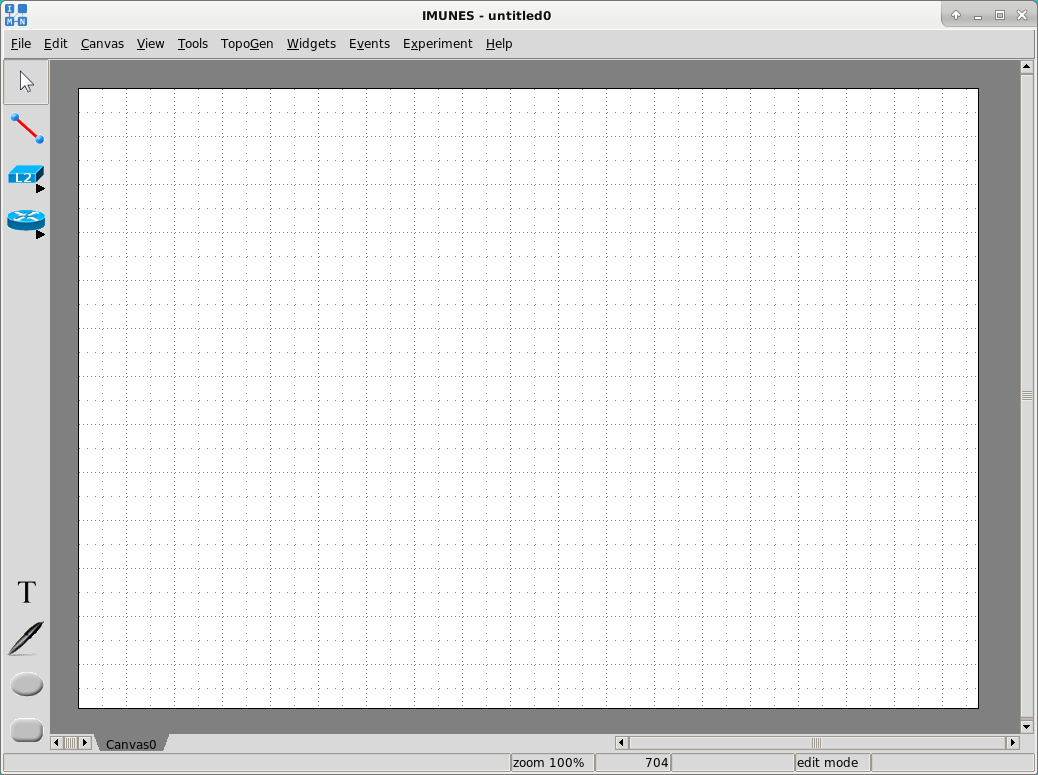
\includegraphics[width=\textwidth]{./images/gui.png}
\caption{\emph{IMUNES GUI}}
\label{fig:imunes_gui}
\end{figure}

The default working mode after the initial start (or after creating a new
virtual network configuration file with the \emph{File $\to$ New} option from
the menubar) is edit mode. The edit mode is used to build and configure network
topologies, contrary to the execute mode whose purpose is the network
simulation. The network simulation will be explained later in the Section
\ref{sec:simulating a simple network}.

\section{Toolbox}
\label{sec:toolbox}
The toolbox, placed on the left side of the GUI, contains tools for building
network topologies and tools for adding annotations (Figure
\ref{fig:toolbox_tools}).These tools are all available in the edit mode. In
the execute mode, these tools (except for the \emph{Select tool}) are shaded
and cannot be used.

\begin{figure}[H]
\centering
\vspace{10pt}
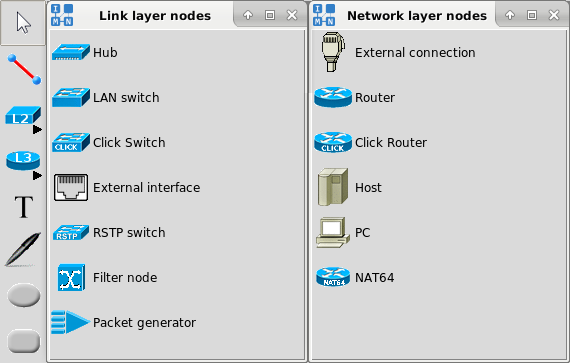
\includegraphics[width=\textwidth]{./images/toolbox.png}
\caption{\emph{Toolbox tools}}
\label{fig:toolbox_tools}
\end{figure}

Each toolbox item shown in Figure \ref{fig:toolbox_tools}, is described below.

  \textbf{Selecting elements:} \hfill
  \begin{itemize}
  \item \emph{Select tool} - The default tool for selecting and moving elements.
  \end{itemize}

  \textbf{Building the network topology:} \hfill
  \begin{itemize}
  \item \emph{Link} - A tool that is used to create network links between nodes.
  \item \textbf{L2 - Link layer nodes (center column):} \hfill
  \begin{itemize}
  \item \emph{Hub} - A link layer element that forwards every incoming packet to all of its ports and, thus, to every connected node.
  \item \emph{LAN switch} - A link layer element that forwards incoming packets to connected nodes using the table of destination addresses and its ports.
  \item \emph{Click switch} - A link layer element that forwards incoming packets to connected nodes using the table of destination addresses and its ports (using Click modular switch).
  \item \emph{External interface} - A tool that provides the possibility to connect a virtual node with the physical interface (e.g. to give the node the access to the Internet).
  \item \emph{RSTP switch} - A Rapid Spanning Tree Protocol switch that can prevent bridge loops and allow providing backup links if an active link fails.
  \item \emph{Filter node} - A link layer element that can filter/divert/forward packets depending on their content.
  \item \emph{Packet generator} - A link layer element to craft custom packets and send them with given packet rate.
  \end{itemize}
  \item \textbf{L3 - Network layer nodes (right column):} \hfill
  \begin{itemize}
  \item \emph{External connection} - A tool that provides the possibility to connect your host PC with a virtual node by creating an interface on your computer.
  \item \emph{Router} - A network layer element that is capable of packet forwarding using the routes obtained by dynamic routing protocols (available through quagga or xorp by default installation or any other standard FreeBSD routing daemon).
  \item \emph{Click Router} - A network layer element that is capable of packet forwarding using the routes obtained by dynamic routing protocols (using Click modular router).
  \item \emph{Host} - A network layer element that does not forward packets and has static routes. It starts standard network services, via portmap and inetd.
  \item \emph{PC} - A network layer element that also does not forward packets and has static routes. Unlike host, it does not start any network services.
  \item \emph{NAT64} - A router node which is capable to enable translation between IPv4 and IPv6 protocols using a form of network address translation (NAT).
  \end{itemize}
  \end{itemize}

  \textbf{Adding annotations:} \hfill
  \begin{itemize}
  \item \emph{Text} - A tool for adding new text on the canvas.
  \item \emph{Oval} - A tool for adding a new oval shape on the canvas.
  \item \emph{Rectangle} - A tool for adding a new rectangle shape on the canvas.
  \item \emph{Freeform} - A tool for adding a new freeform shape on the canvas.
  \end{itemize}

  \section{Menubar}
  The menubar consists of menus that provide access to various functions (Figure
  \ref{fig:menubar}). Some options from the menubar are automatically disabled
  in the execute mode.

  \begin{figure}[H]
  \centering
  \vspace{10pt}
  
\includegraphics[width=\textwidth]{./images/menubar.png}
  \caption{\emph{Menubar}}
  \label{fig:menubar}
  \end{figure}

  \subsection{File Menu}
  The \emph{File} menu contains options for configuration files management
(Figure \ref{fig:file_menu}).
  
  \begin{figure}[H]
  \centering
  \vspace{10pt}
  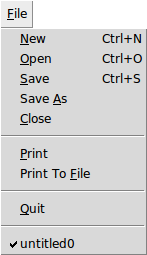
\includegraphics[width=0.21\textwidth]{./images/file_menu.png}
  \caption{\emph{File menu}}
  \label{fig:file_menu}
  \end{figure}
  
  \begin{itemize}
  \item \emph{New} - Create a new virtual network configuration file.
  \item \emph{Open} - Open an existing IMUNES network configuration file (.imn)
by selecting it from the invoked \emph{File Open} dialog.
  \item \emph{Save}, \emph{Save As} - Save the current virtual network topology
in IMUNES network configuration file format (.imn).
  \item \emph{Print} - Print the current canvas using Tcl/Tk PostScript and
send it through the pipe to the default printing command (\emph{lpr}) (that can
also be changed, (e.g > \emph{filename})).
  \item \emph{Print to file} - Print all canvases to PDF or PostScript file. 
  \item \emph{Close} - Close the virtual network configuration file. NOTE: If
the experiment is not explicitly terminated it remains running.
  \item \emph{Quit} - Exit the IMUNES GUI.
  \item \emph{Recently used files} - A list of recently used files. Clicking on
one of the files opens that configuration file.
  \end{itemize}
  
   \subsection{Edit Menu}
  The \emph{Edit} menu contains options for handling elements on the canvas.
  
  \begin{figure}[H]
  \centering
  \vspace{10pt}
  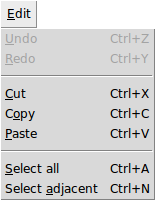
\includegraphics[width=0.23\textwidth]{./images/edit_menu.png}
  \caption{\emph{Edit menu}}
  \label{fig:edit_menu}
  \end{figure}
  
  \begin{itemize}
  \item \emph{Undo} - Undo the last change on the canvas reverting it to an
older state.
  \item \emph{Redo} - Reverse the undo command.
  \item \emph{Cut}, \emph{Copy}, \emph{Paste} - Cut or copy elements from
source and paste them to destination.
  \item \emph{Select all} - Select a whole network topology.
  \item \emph{Select adjacent} - Select nodes connected to the selected
node(s). This feature is also available through the node menu.
  \end{itemize}
  \subsection{Canvas Menu}
  The \emph{Canvas} menu contains options for canvas management.
  
  \begin{figure}[H]
  \centering
  \vspace{10pt}
  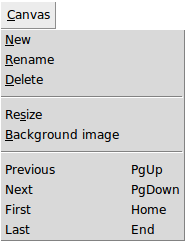
\includegraphics[width=0.26\textwidth]{./images/canvas_menu.png}
  \caption{\emph{Canvas menu}}
  \label{fig:canvas_menu}
  \end{figure}
  
  \begin{itemize}
  \item \emph{New} - Create a new empty canvas.
  \item \emph{Rename} - Rename the current canvas through the invoked dialog.
  \item \emph{Delete} - Delete the current canvas.
  \item \emph{Resize} - Resize the current canvas through the invoked dialog.
  \item \emph{Background image} - Change background on the current canvas (see
Section \ref{sec:CanvasBackgroundImage}).
  \item \emph{Previous, Next, First, Last} - Switch between available canvases.
  \end{itemize}
  
  \subsection{View Menu}
  The \emph{View} menu contains options for showing / hiding links and nodes
parameters on the canvas, options for changing icon size, zooming options, etc.
  
  \begin{figure}[H]
  \centering
  \vspace{10pt}
  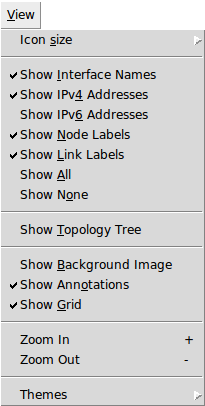
\includegraphics[width=0.29\textwidth]{./images/view_menu.png}
  \caption{\emph{View menu}}
  \label{fig:view_menu}
  \end{figure}
  
  \begin{itemize}
  \item \emph{Icon size} - Change the size (normal or small) of all network
elements (see Section \ref{sec:Icons}).  
  \item \emph{Show [network element parameter]} - Show or hide information such
as interface names, IPv4/IPv6 addresses, etc. These options are usually saved
in the .imn files, providing consistent look of scenarios running on different
computers.
%  \item \emph{Show IPsec Config} - Show or hide information about IPsec
%configuration in the configuration window of network layer elements.
%  \item \emph{Show ZFS snapshots} - Show or hide the configuration of different
%  virtual images from network layer nodes.
  \item \emph{Show Topology Tree} - Show or hide the tree with a list of all
network topology elements.
  \item \emph{Show Background Image} - Show or hide background image.
  \item \emph{Show Annotations} - Show or hide annotations (text, oval,
rectangle).
  \item \emph{Show Grid} - Show or hide grid.
  \item \emph{Zoom In, Zoom Out} - Magnify (\emph{Zoom In}) or reduce
(\emph{Zoom Out}) the size of the display. 
  \item \emph{Themes} - Choose one of the themes from the submenu. Each theme
represents a collection of styles, where a style describes the appearance (or
appearances) of a Ttk widget class.
  \end{itemize}
  
  \subsection{Tools Menu}
  The \emph{Tools} menu contains the network topology management tools.
  
  \begin{figure}[H]
  \centering
  \vspace{10pt}
  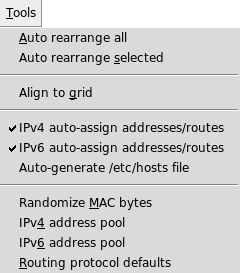
\includegraphics[width=0.25\textwidth]{./images/tools_menu.png}
  \caption{\emph{Tools menu}}
  \label{fig:tools_menu}
  \end{figure}
  
  \begin{itemize}
  \item \emph{Auto rearrange all} - Automatically rearrange position of all
network elements on canvas.
  \item \emph{Auto rearrange selected} - Automatically rearrange position of
the selected group of network elements.
  \item \emph{Align to grid} - Arrange all network elements on canvas aligning
them to grid.
  \item \emph{IPv4 auto-assign addresses/routes} - Automatically assign IPv4
addresses and routes upon creating a new node.
  \item \emph{IPv6 auto-assign addresses/routes} - Automatically assign IPv6
addresses and routes upon creating a new node.
  \item \emph{Auto-generate /etc/hosts file} - Create a \emph{hosts} file on
every node and map every other node hostname with its address.
  \item \emph{Randomize MAC bytes} - Randomizes the 4th and 5th byte of the
automatically generated MAC address.
  \item \emph{IPv4 address pool} - Set variable-mask IPv4 address pool through
the invoked dialog in order to replace default 10.0.0.0/24 address pool (see
Section \ref{sec:IPv4AddressPool}). This will be applied to all the
subsequentially created network layer elements. 
  \item \emph{IPv6 address pool} - Set variable-mask IPv6 address pool through
the invoked dialog in order to replace default fc00::/64 address pool (see
Section \ref{sec:IPv6AddressPool}). This will be applied to all the
subsequentially created network layer elements. 
  \item \emph{Routing protocol defaults} - Set the routing protocol defaults
(routing model and protocols) through the invoked dialog (see Section
\ref{sec:RoutingProtocolDefaults}). This will be applied to all selected
routers (if any) at the time of change, as well as to all the subsequentially
created ones.
  \end{itemize}
  
  \subsection{Topogen Menu}
  The \emph{TopoGen} menu contains options for simple and fast specification of
various network topologies (see Section \ref{sec:GeneratingNetworkTopology}).
  
  \begin{figure}[H]
  \centering
  \vspace{10pt}
  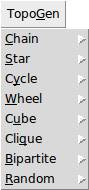
\includegraphics[width=0.13\textwidth]{./images/topogen_menu.png}
  \caption{\emph{Topogen menu}}
  \label{fig:topogen_menu}
  \end{figure}
  
 \subsection{Widgets Menu}
  The \emph{Widgets} menu contains options for displaying information about the
virtual network. To see these information, place the mouse pointer on the
virtual node of interest after selecting a widget.

 \begin{figure}[H]
  \centering
  \vspace{10pt}
  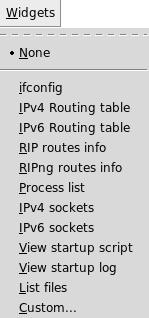
\includegraphics[width=0.17\textwidth]{./images/widgets_menu.png}
  \caption{\emph{Widgets menu}}
  \label{fig:widgets_menu}
  \end{figure}

 \begin{itemize}
 \item \emph{None} - Do not show any information about the virtual network.
 \item \emph{ifconfig} - Show network interfaces parameters.
 \item \emph{IPv4 Routing table} - Show the IPv4 routing table.
 \item \emph{IPv6 Routing table} - Show the IPv6 routing table.
 \item \emph{RIP routes info} - Show the RIP routing information.
 \item \emph{RIPng routes info} - Show the RIPng routing information.
 \item \emph{Process list} - Show the running processes.
 \item \emph{IPv4 sockets} - Show the IPv4 sockets.
 \item \emph{IPv6 sockets} - Show the IPv6 sockets.
 \item \emph{View startup script} - Show the startup script /boot.conf
 \item \emph{View startup log} - Show the startup log /out.log
 \item \emph{Custom...} - Allows the specification of the command that will be
executed inside a virtual node upon placing the mouse pointer on the virtual
node. The result of the command will be displayed inside the widget. 
 \end{itemize}

 \subsection{Events Menu}
 The \emph{Events} menu - This menu is used to configure event scheduling. The
 event scheduling will be explained later in the Section
 \ref{sec:using event scheduler}.

 \begin{figure}[H]
  \centering
  \vspace{10pt}
  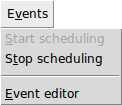
\includegraphics[width=0.18\textwidth]{./images/events_menu.png}
  \caption{\emph{Events menu}}
  \label{fig:events_menu}
  \end{figure}

 \begin{itemize}
 \item \emph{Start scheduling} - Start the scheduling of events.
 \item \emph{Stop scheduling} - Stop the scheduling of events.
 \item \emph{Event editor} - Schedule events on the links through the opened
editor.
 \end{itemize}

  \subsection{Experiment Menu}
  The \emph{Experiment} menu is used to start and terminate an experiment. It
  also enables to attach to a running experiment.
  
  \begin{figure}[H]
  \centering
  \vspace{10pt}
  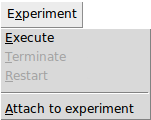
\includegraphics[width=0.21\textwidth]{./images/experiment_menu.png}
  \caption{\emph{Experiment menu}}
  \label{fig:experiment_menu}
  \end{figure}
  
  \begin{itemize}
  \item \emph{Execute} - Start an experiment and switch to the execute mode. In
the process of starting an experiment, IMUNES creates and configures the
virtual network. All events during that process will be shown in the statusbar.
  \item \emph{Terminate} - Terminate an experiment and switch to the edit mode.
During the termination process, IMUNES will shut down all network elements and
it will terminate active services on each node. The termination is finished
when the message about the successful cleanup shows up in the statusbar.
  \item \emph{Restart} - Terminate and restart the running experiment.
  \item \emph{Attach to experiment} - This option opens opens a window with the
list of running experiments on the current computer. It allows to resume
running experiments that are shown in the \emph{Attach to experiment} window
shown in Figure \ref{fig:attach_to_experiment}.
  \end{itemize}
  
  \subsection{Help Menu}
  The \emph{Help} menu contains the option \emph{About} that invokes the
\emph{About} dialog box for viewing version information.
  
  \begin{figure}[H]
  \centering
  \vspace{10pt}
  
\includegraphics[width=0.09\textwidth]{./images/help_menu.png}
  \caption{\emph{Help menu}}
  \label{fig:help_menu} \end{figure}
   

   \chapter{Quick Intro}

\section{Simple Network Scenario}
\label{sec:SimpleNetworkScenario}
In this section we will show how to build, configure and simulate the following
simple network topology:

Personal computers (\emph{office-pc1} and \emph{office-pc2}) from the network
192.168.1.0/24 are connected to the LAN switch (\emph{office-switch}) which is
connected to the router (\emph{office-router}). The server (\emph{office-host})
from the network 192.168.2.0/24 is directly connected to the router
(\emph{office-router}). Personal computers from the first network have route
only to the network 192.168.2.0/24. The server from the second network has the
default route. Quagga routing is enabled on the router in order to be able to
serve and receive dynamic route updates.

\subsection{Building a simple network}
After running IMUNES on FreeBSD with some kind of X11 window manager (see
Section \ref{sec:UserInterfaceLayout}), we will build previously described
network using tools from the toolbox (see Section \ref{sec:toolbox}).

\subsubsection{Adding and deleting network elements}
To draw a node click on the corresponding node tool and then click on the
workspace to place it. To connect nodes click on the \emph{Link tool}, then
click and hold on the source node and go to the destination node.

Now draw a router, a host, a LAN switch and two PCs. Using the \emph{Link tool}
connect the LAN switch to the router and then connect each PC to the LAN
switch. Connect the host directly to the router. The created network topology
should look like the one in Figure \ref{fig:simple_topology}.

\begin{figure}[H]
\centering
\vspace{10pt}
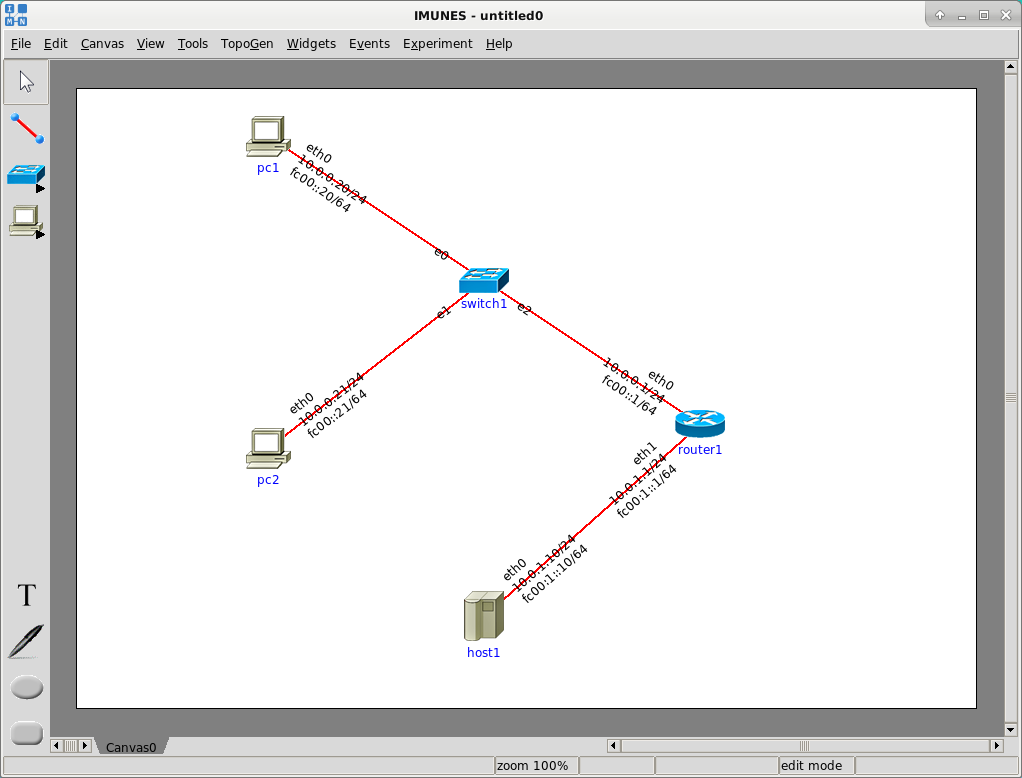
\includegraphics[width=\textwidth]{./images/simple_topology.png}
\caption{\emph{Simple network topology}}
\label{fig:simple_topology}
\end{figure}

When nodes are connected with the \emph{Link tool} (the direction does not
matter), the source node, the destination node and the link automatically get
preconfigured parameters. When a mouse pointer is above a node or a link, some
of the configured parameters are shown on the left side of the statusbar placed
at the bottom of the window (Figure \ref{fig:statusbar_node}).

\begin{figure}[H]
\centering
\vspace{10pt}

\includegraphics[width=\textwidth]{./images/statusbar1.png}
\caption{\emph{Node parameters in the statusbar}}
\label{fig:statusbar_node}
\end{figure}

Some of the parameters can be visible on the canvas: interface names (link
layer: e0, e1, e2 and network layer: eth0, eth1), IPv4/IPv6 addresses of
network layer elements (PC, host, router), node names (router1, host1, switch1,
pc1, pc2) and link labels (Bandwidth, Delay, BER or Duplicate if their values
are not default).

You can manipulate with the visibility of nodes and links parameters from the
View menu (Figure \ref{fig:view_menu1}). In this simple scenario we do not want
for IPv6 addresses to be visible, so we will turn the \emph{Show IPv6
Addresses} option off.

\begin{figure}[H]
\centering
\vspace{10pt}
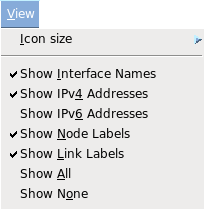
\includegraphics[width=0.28\textwidth]{./images/view_menu1.png}
\caption{\emph{Show or hide nodes and links parameters}}
\label{fig:view_menu1}
\end{figure}

To delete the network element select it using the \emph{Select tool} and then
use the \emph{Delete} keyboard button. You can also delete it by right clicking
on it and clicking on the \emph{Delete} label in the popped up menu. The node
deletion is automatically followed by the deletion of associated links.

\subsubsection{Rearranging network elements}
You can change position of the network element (node or link) and/or the node
name. To move both the network element and its name select the network element
with the \emph{Select tool} and drag it to the designated position. To move
only the node name select it with the \emph{Select tool} and drag it to the
designated position.

Using the \emph{Select tool} you can also move around a group of connected
nodes which can be selected using the \emph{Ctrl} keyboard button in addition
to the left click. To select the whole network topology use \emph{Select All}
option from the \emph{Edit} menu.

For automatic rearranging of all network elements or rearranging the selected
group of network elements use \emph{Rearrange} and \emph{Rearrange All} options
from the \emph{Tools} menu. To stop the rearranging process click with the
\emph{Select tool}.

\subsection{Configuring a simple network}

Although preconfigured parameters of network elements are usually sufficient to
start a simulation (automatically provided IPv4/IPv6 addresses, the default
static route on the PC and the host and routing model and protocols parameters
on the router as well), in this scenario we will set up our own parameters.

To open the network element configuration window:
\begin{itemize}
  \item right click on the network element and select the \emph{Configure}
label from the popped up menu (Figure \ref{fig:configure_label}) 
  
  or
  
  \item double click on the network element.
\end{itemize}

\begin{figure}[H]
\centering
\vspace{10pt}
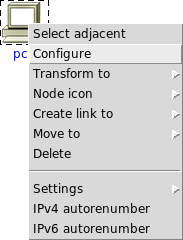
\includegraphics[width=0.28\textwidth]{./images/configure_label.png}
\caption{\emph{Configure a network element}}
\label{fig:configure_label}
\end{figure}

Network elements configuration parameters can be also changed through the
topology tree. To show the topology tree turn on the \emph{Show Topology Tree}
option from the \emph{View} menu. The tree with a list of network topology
elements (nodes and links) will be shown on the right side of the window
(Figure \ref{fig:topology_tree}). To open the network element configuration
window double click or use the \emph{Enter} keyboard button on node, interface
or link label in the topology tree.

\begin{figure}[H]
\centering
\vspace{10pt}
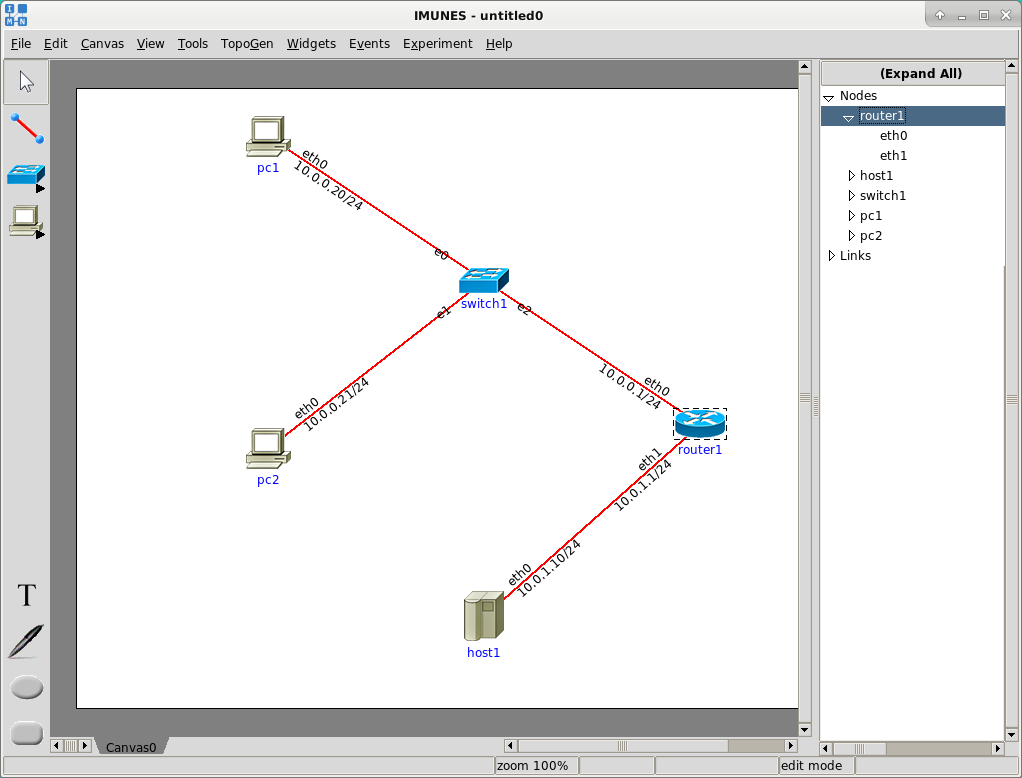
\includegraphics[width=\textwidth]{./images/topology_tree.png}
\caption{\emph{Changing configuration parameters through the topology tree}}
\label{fig:topology_tree}
\end{figure}

Depending on the type of a network element in our topology, there are 4 types
of configuration windows:

\begin{itemize}
  \item \emph{Hub/LAN switch configuration} window
  \item \emph{PC/Host/Click router configuration} window
  \item \emph{Router configuration} window
  \item \emph{Link configuration} window
\end{itemize}

There are also other types of configuration windows which are explained in
other sections:

\begin{itemize}
  \item \emph{External interface configuration} window
  \item \emph{External connection configuration} window
  \item \emph{NAT64 configuration} window
  \item \emph{RSTP switch configuration} window
  \item \emph{Filter node configuration} window
  \item \emph{Packet generator configuration} window
  \item \emph{Click switch configuration} window
\end{itemize}

\subsubsection{Hub/LAN switch configuration window}
The \emph{hub/LAN switch configuration} window, as well as the configuration
windows of other node types, contains a node name field. Besides that it
contains only link layer interface parameters.

We will change the LAN switch name and data packet scheduling method (from
preconfigured First In First Out (FIFO) data packet scheduling method to
Weighted Fair Queuing (WFQ) method).

Change the node name to \emph{office-switch}.
To change data packet scheduling method select the link layer interface
\emph{e0} from the list of interfaces, choose \emph{WFQ} option from the
\emph{Queue} menu and click on the \emph{Apply} button (Figure
\ref{fig:LANswitch_config}). 

\begin{figure}[H]
\centering
\vspace{10pt}
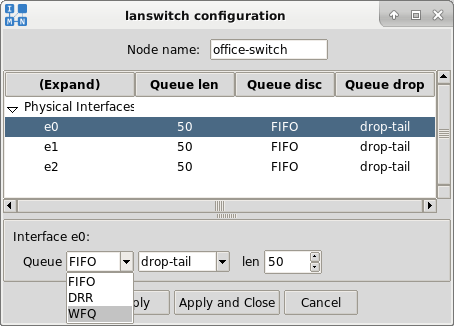
\includegraphics[width=0.6\textwidth]{./images/LANswitch_config.png}
\caption{\emph{LAN switch configuration window}}
\label{fig:LANswitch_config}
\end{figure}

Packet scheduling method is now applied and you can see new queuing discipline
for interface \emph{e0} in the column \emph{Queue disc} (Figure
\ref{fig:LANswitch_config_applied}). 

\begin{figure}[H]
\centering
\vspace{10pt}
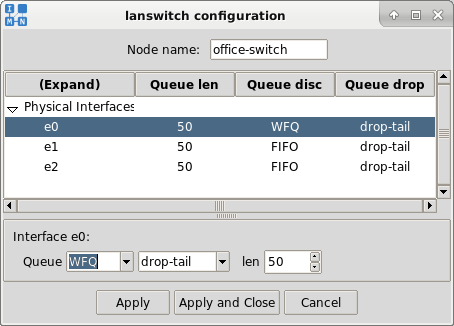
\includegraphics[width=0.6\textwidth]{./images/LANswitch_config_applied.png}
\caption{\emph{LAN switch configuration window with applied changes}}
\label{fig:LANswitch_config_applied}
\end{figure}

Repeat the same procedure for the other link layer interfaces.
Changed configuration is already applied so you can close the configuration
window with the \emph{Cancel} button but you can also use the \emph{Apply and
Close} button.

\subsubsection{PC/Host/Click router configuration window}
The \emph{PC/Host/Click router configuration} window consists of two
subwindows. Each of them is associated with one of the following tabs:
\emph{Configuration} and \emph{Interfaces} (Figure \ref{fig:pc_config_tabs}).

\begin{figure}[H]
\centering
\vspace{10pt}
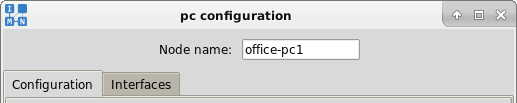
\includegraphics[width=0.6\textwidth]{./images/pc_config_tabs.png}
\caption{\emph{Tabs in the PC/Host/Click router configuration window}}
\label{fig:pc_config_tabs}
\end{figure}

Besides a node name field, \emph{PC/Host/Click router configuration} window
contains startup services, routing parameters and custom configuration
parameters (in the window associated with the \emph{Configuration} tab) and
network interface parameters (in the window associated with the
\emph{Interfaces} tab).

We will change the node name, network interface parameters and routing
parameters.

Change the host node name to \emph{office-host} and PC node names to
\emph{office-pc1} and \emph{office-pc2}.
To change IPv4 address left click on the \emph{Interfaces} tab, select
interface \emph{eth0} from the list of interfaces, change the IPv4 address
field and click on the \emph{Apply} button (Figure \ref{fig:pc_config_ipv4}).
We will change the host IPv4 address field to 192.168.2.5/24 (now it belongs to
192.168.2.0/24) and PC IPv4 address fields to 192.168.1.5/24 and 192.168.1.7/24
(now they belong to network 192.168.1.0/24). IP address fields require the CIDR
notation, so the IPv4 address is followed by a slash and a network length.

\begin{figure}[H]
\centering
\vspace{10pt}
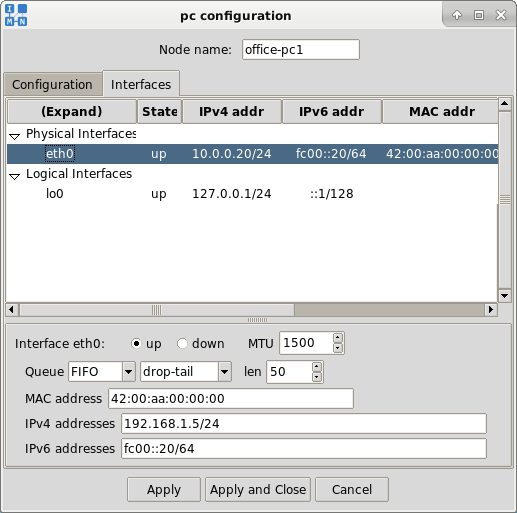
\includegraphics[width=0.6\textwidth]{./images/pc_config_ipv4.png}
\caption{\emph{Changing IPv4 address}}
\label{fig:pc_config_ipv4}
\end{figure}

\paragraph{\emph{Static routes}} \hfill

PCs and Hosts both use static routing. The preconfigured routing table contains
only the default route. Every static route, as well as the default route,
consists of:
\begin{enumerate}
  \item the destination network: an IP address which is followed by a slash and
a network prefix and
  \item the next hop network interface IP address (which is an IP address
without a slash and without a network prefix).
\end{enumerate}

If the route syntax is wrong, that route will be silently ignored. 

We will add the static route on \emph{office-pc1} and \emph{office-pc2} for the
network 192.168.2.0/24 through the gateway 192.168.1.1 (Figure
\ref{fig:pc_config_staticroutes}). 

\begin{figure}[H]
\centering
\vspace{10pt}
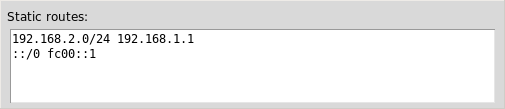
\includegraphics[width=0.6\textwidth]{./images/pc_config_staticroutes.png}
\caption{\emph{Adding the static route on the PC}}
\label{fig:pc_config_staticroutes}
\end{figure}

On \emph{office-host} we will change default gateway address to 192.168.2.1
(Figure \ref{fig:host_config_staticroutes}).

\begin{figure}[H]
\centering
\vspace{10pt}
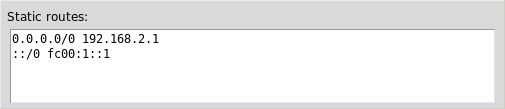
\includegraphics[width=0.6\textwidth]{./images/host_config_staticroutes.png}
\caption{\emph{Adding the static route on the PC}}
\label{fig:host_config_staticroutes}
\end{figure}

IPv6 addresses and default routes (placed below IPv4 addresses and routes) can
be deleted.

To apply the changed configuration and close the configuration window click on
the \emph{Apply and Close} button.

\subsubsection{Router configuration window}
The \emph{router configuration window}, in addition to fields from
\emph{PC/Host/Click router configuration} window, contains the part for
choosing the routing model and protocols, as well as an \emph{IPsec} tab with
IPsec parameters (See IPsec Section TODO).

We will only change the node name and network interface parameters.

Change the node name to \emph{office-router} and IPv4 addresses on both network
interfaces: 192.168.1.1/24 on the network interface \emph{eth0} and
192.168.2.1/24 on the network interface \emph{eth1}.

\paragraph{\emph{Routing models and protocols}} \hfill

There are three possible routing models:
\begin{enumerate}
  \item the quagga model
  \item the xorp model (eXtensible Open Router Platform)
  \item the static model
\end{enumerate}

In the case of quagga and xorp routing models, there are options for
enabling/disabling RIP, RIPng, OSPFv2 and OSPFv3. By default, all new quagga or
xorp router instances will have both RIPv2 and RIPng enabled. The defaults can
be changed with the \emph{Tools $\to$ Routing protocol defaults} option from
the menubar, which will be applied to all selected routers (if any) at the time
of change, as well as to all the subsequentially created ones (see Section
\ref{sec:RoutingProtocolDefaults}).
In the case of static routing model, the router uses routes from the static
routes field that has the same syntax as the static routes field in the
\emph{PC/Host/Click router configuration} window.

We will leave the default router model - quagga with RIP and RIPng protocols
enabled, and OSPFv2 and OSPFv3 protocols disabled (Figure
\ref{fig:router_config_routingmodels}).

\begin{figure}[H]
\centering
\vspace{10pt}
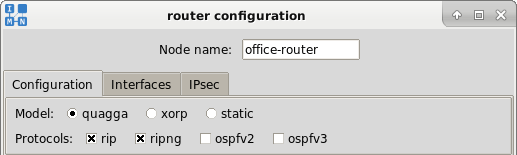
\includegraphics[width=0.6\textwidth]{./images/router_config_routingmodels.png}
\caption{\emph{Routing models and protocols}}
\label{fig:router_config_routingmodels}
\end{figure}

\subsubsection{Link configuration window}
The \emph{link configuration} window offers the possibility to configure the
link bandwidth (between 0 and 10\textsuperscript{9} bps), the propagation delay
(between 0 and 10\textsuperscript{7} $\mu$s), the bit error
rate (between 0 and 10\textsuperscript{12}) and the probability of package
duplication (between 0 and 50\%). There are also display properties: the link
width (line thickness between 1 and 8) and the link color (red, green, blue,
yellow, magenta, cyan or black).

\begin{figure}[H]
\centering
\vspace{10pt}
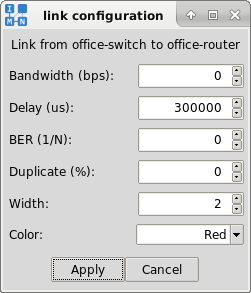
\includegraphics[width=0.4\textwidth]{./images/link_config.png}
\caption{\emph{Link configuration window}}
\label{fig:link_config}
\end{figure}

Default values are as follows: the link which transmits packets without errors
and without any possibility for the packet duplication with the unlimited link
bandwidth and the zero propagation delay. The link width is set to value 2 and
the link color is red.

We will leave default values on all links except on the link between
\emph{office-switch} and \emph{office-router} (Figure
\ref{fig:configured_topology}). On that link we will set up the delay of 30000
$\mu$s. Delay will be tested during the network simulation with the
\emph{traceroute} tool (see Section \ref{sec:NodeandLinkMenuOptions}).

\subsubsection{Configured network topology}
Configured network topology should look like the one in Figure
\ref{fig:configured_topology}.

\begin{figure}[H]
\centering
\vspace{10pt}
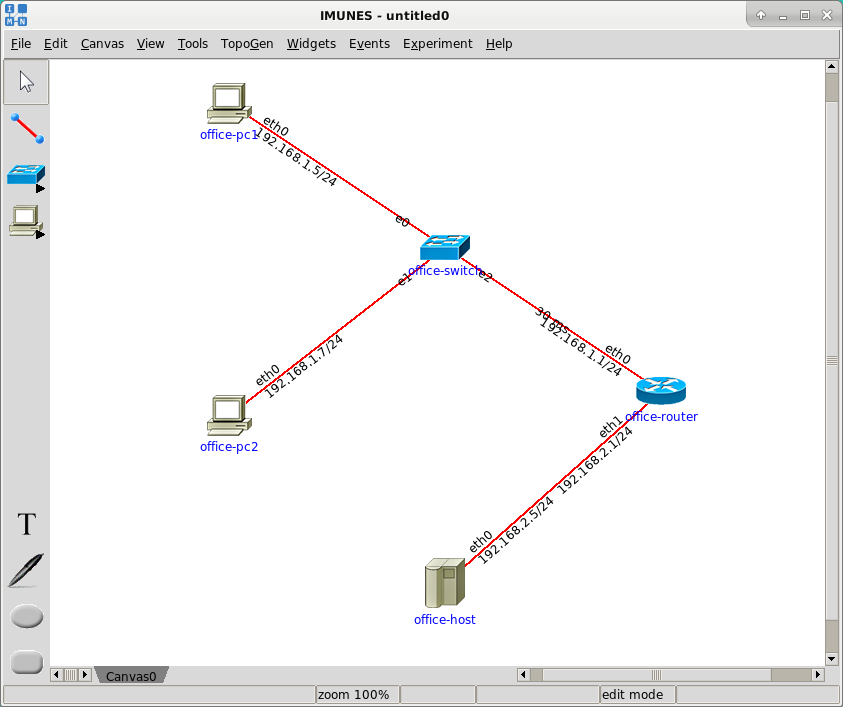
\includegraphics[width=\textwidth]{./images/simple_topology_configured.png}
\caption{\emph{Configured network topology}}
\label{fig:configured_topology}
\end{figure}

\subsection{Simulating a simple network}
\label{sec:simulating a simple network}

\subsubsection{Starting an experiment}
After the network topology is completely built and properly configured, we will
start an experiment with the \emph{Experiment $\to$ Execute}  option from the
menubar and IMUNES will switch from the edit mode to the execute mode. In the
process of starting an experiment, IMUNES creates and configures the virtual
network. That will take a few seconds and all events during that process will
be shown in the statusbar placed at the bottom of the window.

\textbf{NOTE:} Although you can draw network topology on any system that
supports Tcl/Tk (Linux, FreeBSD, Windows, Mac OS X, Solaris), an  experiment
can only be started on FreeBSD and Linux operating systems with root
permissions (Figure \ref{fig:execute_windows} and Figure
\ref{fig:execute_not_root})!

\begin{figure}[H]
\centering
\vspace{10pt}

\includegraphics[width=0.7\textwidth]{./images/execute_windows.png}
\caption{\emph{Starting an experiment in Windows}}
\label{fig:execute_windows}
\end{figure}

\begin{figure}[H]
\centering
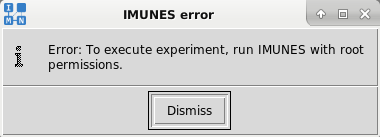
\includegraphics[width=0.5\textwidth]{./images/execute_not_root.png}
\caption{\emph{Starting an experiment in FreeBSD without root permissions}}
\label{fig:execute_not_root}
\end{figure}
 
In addition to configured parameters, each node will be set with the loopback
interface, a router will have the kernel forwarding enabled, and a host node
will have portmap and inetd started.

Information about the time spent instantiating the network topology is shown in
the statusbar (Figure \ref{fig:statusbar_execute}).

\begin{figure}[H]
\centering
\vspace{10pt}

\includegraphics[width=\textwidth]{./images/statusbar3.png}
\caption{\emph{Message about the instantiation of the network topology}}
\label{fig:statusbar_execute}
\end{figure}

In the right corner of the statusbar you can also see that IMUNES now works in
the execute mode, as well as experiment unique identifier.

\subsubsection{Options from the node and the link menu}
\label{sec:NodeandLinkMenuOptions}
To open the node menu in the execute mode right click on the node. Note that
the menu in the execute mode is different from the menu in the edit mode. It
offers the possibility to select the node connected to this node (\emph{Select
adjacent}), to see the current configuration (\emph{Configure}), to \emph{Start
/ Stop / Restart} the network element, to start / stop / restart any of the
possible \emph{Services} or to \emph{Import Running Configuration} from the
\emph{Settings} menu. The \emph{Import Running Configuration} option copies the
current MTU value and IPv4/IPv6 addresses from the running node to its
configuration. It is also possible to open the \emph{Shell window} (X terminal
with a Unix shell), \emph{Wireshark} or \emph{tcpdump} network sniffers on any
of the interfaces, \emph{Firefox} \emph{Web Browser} or a \emph{Mail client}.

\begin{figure}[H]
\centering
\vspace{10pt}
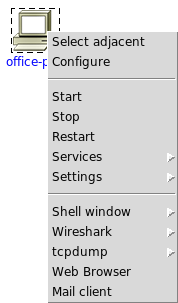
\includegraphics[width=0.28\textwidth]{./images/execute_menu.png}
\caption{\emph{Network-layer node menu in the execute mode}}
\label{fig:execute_menu}
\end{figure}

Note that both the node and the link menu in the execute menu offer the
possibility to open the configuration window (\emph{Configure} label). 

From the node configuration window in the execute mode it is possible to change
only the node name. Other node parameters such as link layer interface
parameters, network interface parameters and routing parameters can be changed
from the shell window on each node. To change those parameters from the node
configuration window, stop the node (using the \emph{Stop} label), change
parameters and then start the node agin (using the \emph{Start} label).

On the other side, from the link configuration window in the execute mode it is
possible to change the following link parameters: link bandwidth, the
propagation delay, the bit error rate and the probability of package
duplication. It is also possible to change display properties: the link
width and the link color.

We will now check if the virtual network topology is properly configured. Open
the shell window (e.g. \emph{Shell window} $\to$ \emph{csh} or simply double
click on the node) on the network element (e.g. \emph{office-pc1}).
\begin{itemize}
\item To check the network interface eth0 parameters type the following
command: \texttt{ifconfig eth0}. The result is shown in Figure
\ref{fig:pc_ifconfig}.

\begin{figure}[H]
\centering
\vspace{10pt}
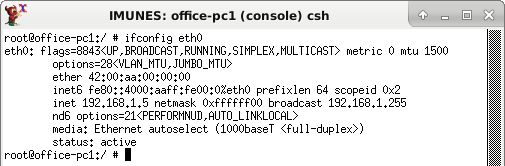
\includegraphics[width=0.8\textwidth]{./images/pc_ifconfig.png}
\caption{\emph{Shell window on office-pc1, network interface parameters}}
\label{fig:pc_ifconfig}
\end{figure}

\item To check static routes type the following command: \texttt{netstat -nrf
inet}. The result is shown in Figure \ref{fig:pc_netstat}.

\begin{figure}[H]
\centering
\vspace{10pt}
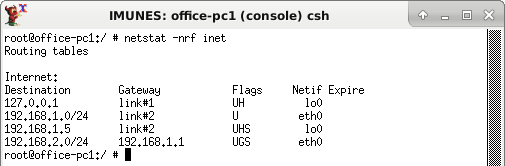
\includegraphics[width=0.8\textwidth]{./images/pc_netstat.png}
\caption{\emph{Shell window on office-pc1, static routes}}
\label{fig:pc_netstat}
\end{figure}

\item To test if a particular network element is reachable (e.g
\emph{office-host}) type the following command: \texttt{ping 192.168.2.5}. The
result is shown in Figure \ref{fig:pc_ping}. To stop transmitting packets press
\emph{Control-C} keyboard button.

\begin{figure}[H]
\centering
\vspace{10pt}
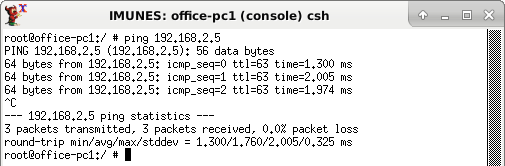
\includegraphics[width=0.8\textwidth]{./images/pc_ping.png}
\caption{\emph{Shell window on office-pc1, pinging office-host}}
\label{fig:pc_ping}
\end{figure}

\end{itemize}

We will test delay on the link between \emph{office-switch} and
\emph{office-router}, which is set to 30000 $\mu$s (30 ms), by using the
\emph{traceroute} tool:
\begin{itemize}
\item In the shell window on \emph{office-pc1} type the following command: \\
\texttt{traceroute 192.168.1.1}. The result is shown in Figure
\ref{fig:pc_traceroute}.

\begin{figure}[H]
\centering
\vspace{10pt}
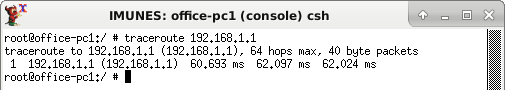
\includegraphics[width=0.8\textwidth]{./images/pc_traceroute.png}
\caption{\emph{Shell window on office-pc1, traceroute to office-router}}
\label{fig:pc_traceroute}
\end{figure}

\item In the shell window on \emph{office-host} type the following command: \\
\texttt{traceroute 192.168.2.1}. The result is shown in Figure
\ref{fig:host_traceroute}.

\begin{figure}[H]
\centering
\vspace{10pt}
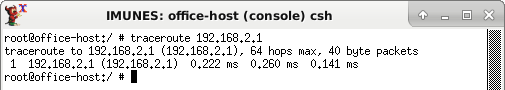
\includegraphics[width=0.8\textwidth]{./images/host_traceroute.png}
\caption{\emph{Shell window on office-host, traceroute to office-router}}
\label{fig:host_traceroute}
\end{figure}

\end{itemize}

\subsubsection{Terminating an experiment}
To terminate an experiment and switch from the execute mode to the edit mode
use the \emph{Experiment $\to$ Execute} option from the menubar. During the
termination process, IMUNES will terminate active services on each node and
shut down all network elements (links and nodes with both virtual and physical
interfaces). The termination is finished when the message about the successful
cleanup shows up in the statusbar (Figure \ref{fig:statusbar4}).

\begin{figure}[H]
\centering
\vspace{10pt}

\includegraphics[width=\textwidth]{./images/statusbar4.png}
\caption{\emph{Message about the successful cleanup}}
\label{fig:statusbar4}
\end{figure}

\section{Configuration files management}

\subsection{Saving a virtual network configuration}

After the virtual network is successfully built, configured and tested, it can
be saved with \emph{File $\to$ Save} or \emph{File $\to$ Save As} options from
the menubar. The virtual network topology is saved in IMUNES network
configuration file format (.imn).

\begin{figure}[H]
\centering
\vspace{10pt}
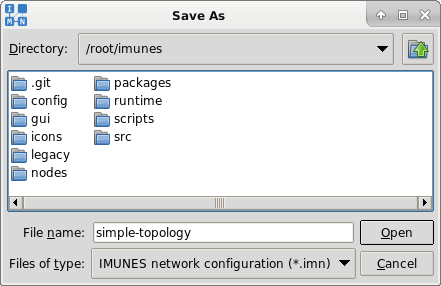
\includegraphics[width=0.65\textwidth]{./images/file_save.png}
\caption{\emph{File Save dialog}}
\label{fig:file_save}
\end{figure}

The structure of the configuration file is simple and suitable for changing
with a text editor (see Appendix \ref{sec:IMUNESNetworkConfigurationFile}).

\subsection{Opening a virtual network configuration}
To open an existing IMUNES network configuration file use the \emph{File $\to$
Open} option from the menubar and select it from the invoked \emph{File Open}
dialog. 

\begin{figure}[H]
\centering
\vspace{10pt}
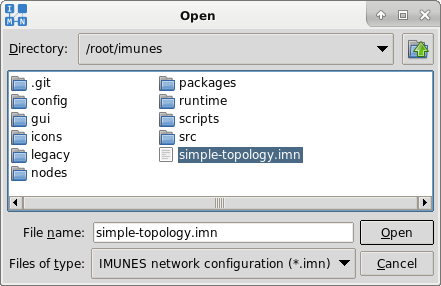
\includegraphics[width=0.65\textwidth]{./images/file_open.png}
\caption{\emph{File Open dialog}}
\label{fig:file_open}
\end{figure}

The other way to open an imn file is to start IMUNES with that file as an
argument: \texttt{imunes simple-topology.imn}

   \chapter{Advanced Usage}
\section{Extended Network Scenario}
In this section we will show how to extend the simple network topology (see
Section \ref{sec:SimpleNetworkScenario}). We will explain the additional
possibilities of building and configuring the extended network scenario:

The simple network topology is placed in the \emph{office-canvas} while the
additional elements are placed in the \emph{roadwarrior-canvas}. The
\emph{roadwarrior-canvas} consists of a router (\emph{roadwarrior-router}), a
PC (\emph{roadwarrior}) and a physical interface. The \emph{roadwarrior-router}
is connected to the \emph{office-router} on the \emph{office-canvas} through
the 192.168.3.0/24 network, the PC is in the 161.53.19.0/24 network whereas the
physical interface is in the 161.53.20.0/24 network.

We will now extend the simple network from the last chapter by adding the
\emph{roadwarrior-router}, \emph{roadwarrior} and the physical interface all
placed on another canvas. To open an existing IMUNES network configuration file
use \emph{File $\to$ Open} from the menubar or start IMUNES with the imn file
as an argument: \texttt{imunes simple-topology.imn}. Check that you are in the
edit mode. If not, switch with \emph{Experiment $\to$ Terminate}.

\subsection{Canvas Management}
To facilitate building of complex and large network topologies IMUNES lets you
divide the network topology into a set of network layers. These network layers
are called canvases.

Canvas management consists of two main elements:
\begin{itemize}
    \item Canvas menu in the menubar (Figure \ref{fig:canvas_menu})
    \item List of canvas tabs at the bottom of the main window, above the
statusbar (Figure \ref{fig:canvas_tabs_list})
    \begin{figure}[H]
	\centering
	\vspace{10pt}
	
\includegraphics[width=0.55\textwidth]{./images/canvas_tabs_list.png}
	\caption{\emph{Canvas Tabs}}
	\label{fig:canvas_tabs_list}
    \end{figure}
\end{itemize}

To add a new canvas use the \emph{Canvas $\to$ New} option from the menubar or
double click on the empty space in the canvas tabs list at the bottom of the
window.

You can rename the canvas with the \emph{Canvas $\to$ Rename} option from the
menubar or double click on the canvas tab in the canvas tabs list. (Figure
\ref{fig:canvas_rename}) Similarly the \emph{Canvas $\to$ Delete} option
deletes the active canvas.
\begin{figure}[H]
    \centering
    \vspace{10pt}
    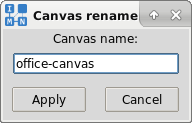
\includegraphics[width=0.25\textwidth]{./images/canvas_rename.png}
    \caption{\emph{Canvas rename dialog}}
    \label{fig:canvas_rename}
\end{figure}

There is also the option \emph{Canvas $\to$ Resize} that allows you to define a
custom canvas size in pixels. The default canvas size is 900*620 pixels.
(Figure \ref{fig:canvas_resize})
\begin{figure}[H]
    \centering
    \vspace{10pt}
    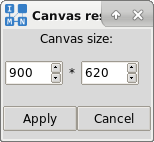
\includegraphics[width=0.20\textwidth]{./images/canvas_resize.png}
    \caption{\emph{Canvas resize dialog}}
    \label{fig:canvas_resize}
\end{figure}

Canvas selection can be done with the options from the \emph{Canvas} menu
(\emph{Previous, Next, First, Last}) or simply by clicking the tab with the
canvas name on it.

Rename the existing canvas \emph{Canvas0} into \emph{office-canvas}. Add a new
canvas, rename it into \emph{roadwarrior-canvas} and select it as the active
canvas. 

This canvas is empty so we will add a router by selecting the router tool and
clicking on the empty canvas. Rename this router into
\emph{roadwarrior-router}. Switch to the \emph{office-canvas}.  Now we will
connect the \emph{office-router} and the \emph{roadwarrior-router}. To do that,
right click on the \emph{office-router} and select \emph{Create link to $\to$
roadwarrior-canvas $\to$ roadwarrior-router} option (Figure
\ref{fig:create_link_to}) from the popped up menu. This will create a link
between \emph{roadwarrior-router} and \emph{office-router}.
\begin{figure}[H]
    \centering
    \vspace{10pt}
    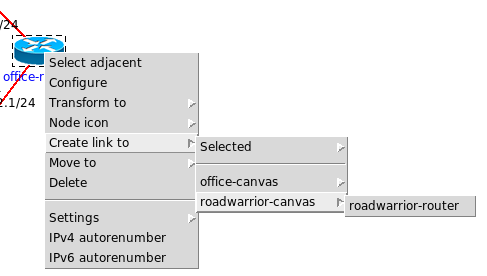
\includegraphics[width=0.65\textwidth]{./images/create_link_to.png}
    \caption{\emph{Create link to}}
    \label{fig:create_link_to}
\end{figure}

On the \emph{office-router} set the \emph{eth2} interface IPv4 address to
192.168.3.1/24. On the \emph{roadwarrior-router} set the \emph{eth0} interface
IPv4 address to 192.168.3.2/24.  We will add another PC to the
\emph{roadwarrior-canvas}, name it \emph{roadwarrior} and connect it with the
\emph{roadwarrior-router}. On the \emph{roadwarrior} set the eth0 IPv4 address
to 161.53.19.100/24. On the \emph{roadwarrior-router} set the eth1 IPv4 address
to 161.53.19.1/24.

The \emph{roadwarrior-router} uses the same dynamic routing model (quagga) as
the \emph{office-router} and we do not need to configure anything else on the
router. The \emph{roadwarrior} uses static routes and we will need to change
the default route gateway in static routes field of the \emph{roadwarrior}
configuration window to 0.0.0.0/0 161.53.19.1.

Finally, the configured network topology should look like the following (Figure
\ref{fig:office_canvas} and Figure \ref{fig:roadwarrior_canvas}):

\begin{figure}[H]
    \centering
%     \vspace{10pt}
    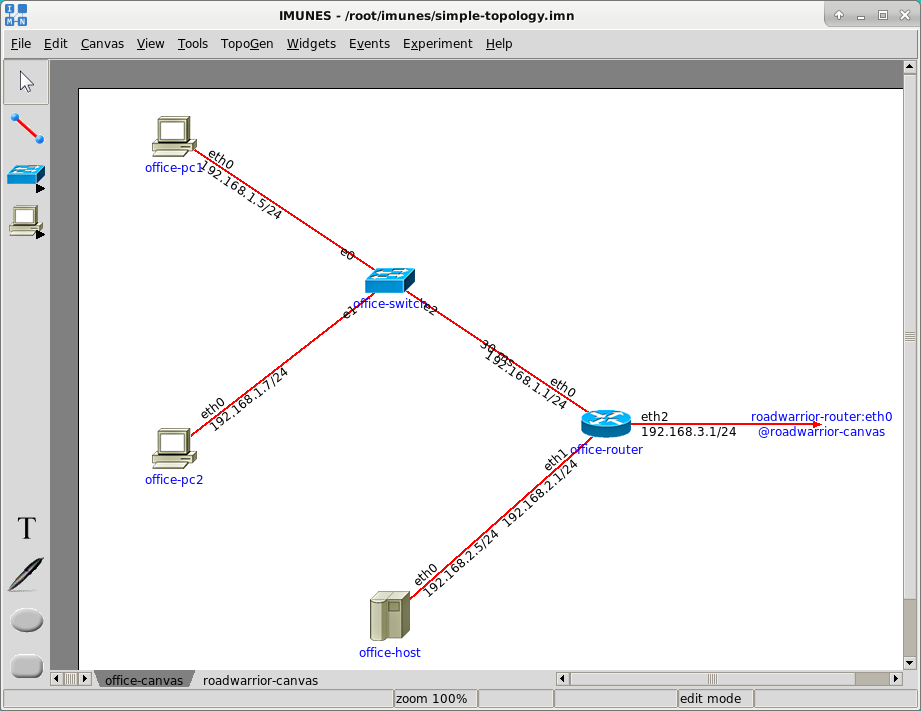
\includegraphics[width=\textwidth]{./images/office_canvas.png}
    \caption{\emph{office-canvas}}
    \label{fig:office_canvas}
\end{figure}

\begin{figure}[H]
    \centering
%     \vspace{10pt}
    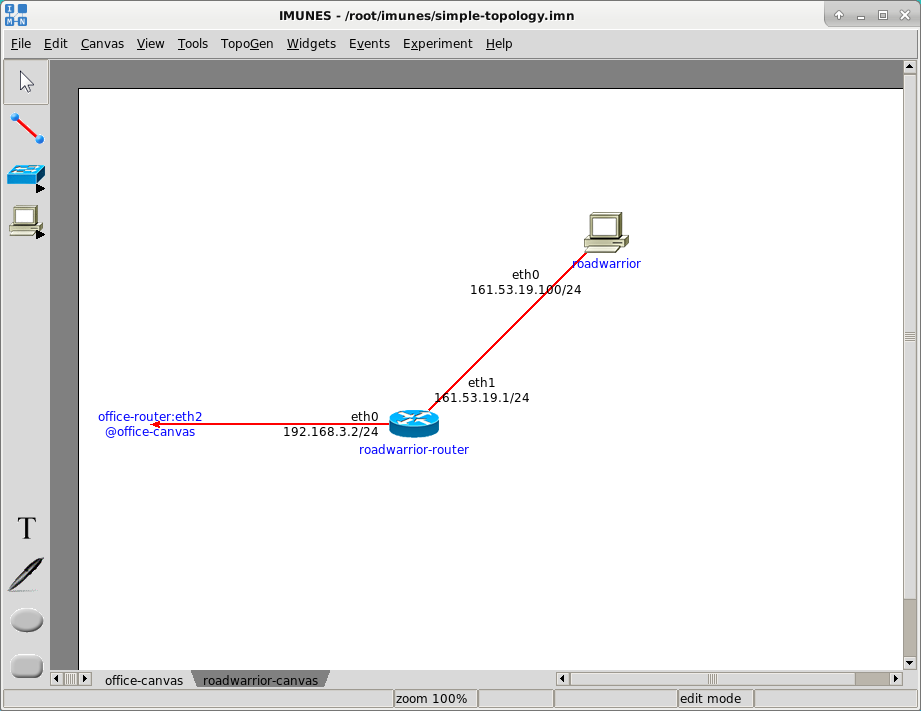
\includegraphics[width=\textwidth]{./images/roadwarrior_canvas.png}
    \caption{\emph{roadwarrior-canvas}}
    \label{fig:roadwarrior_canvas}
\end{figure}
 

Both the \emph{roadwarrior} and \emph{roadwarrior-router} can be easily moved
from \emph{roadwarrior-canvas} to \emph{office-canvas} with the \emph{Move To
$\to$ office-canvas} from the node menu. The link between
\emph{roadwarrior-router} and \emph{office-router}, as well as any other link,
can be deleted with the \emph{Delete} option from the \emph{Link} menu. To open
the \emph{link} menu, use the right click on the link and choose the
\emph{Delete} option.

When we are done with network configuration, we can start the experiment with
\emph{Experiment $\to$ Execute} from the menubar. We can now check that the
\emph{roadwarrior} can ping both networks (192.168.1.0/24, 192.168.2.0/24) and
additionally, that the network 192.168.1.0/24 does not have an access to the
\emph{roadwarrior}, but it has access to the 192.168.2.0/24 network.

\subsection{Attaching an external interface}

The \emph{External interface} tool from the toolbox provides the possibility to
attach a physical interface to a virtual node. This way the virtual network is
able to communicate with nodes from the external network.

We will now add the external interface to the \emph{roadwarrior-canvas}. To add
a external interface to the canvas select the \emph{External interface} tool
and click on the canvas.

\emph{External interface} nodes can be connected either with the LAN switch or the
router. Connect the newly created external interface with the virtual node
\emph{roadwarrior-router} using the \emph{Link} tool from the toolbox or the
\emph{Create link to} option from the node menu.

The newly created external interface node is unassigned and in the node name
field it contains \emph{UNASSIGNED}. Open the external interface configuration
window with a double click or right click on it and select the \emph{Configure}
option. Choose the name of the designated physical interface in the
\emph{Physical interface} drop-down list, e.g. em1, obtained from
\texttt{ifconfig -a} command ran on the physical machine (outside IMUNES).
(Figure \ref{fig:rj45_conf}) The name of the physical interface will appear in
the node name label. It is also possible to assign a VLAN tag to it. (Figure
\ref{fig:rj45_canvas})

\begin{figure}[H]
    \centering
%     \vspace{10pt}
    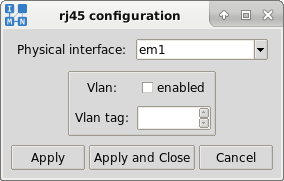
\includegraphics[width=0.37\textwidth]{./images/rj45_conf.png}
    \caption{\emph{External interface configuration dialog}}
    \label{fig:rj45_conf}
\end{figure}

\begin{figure}[H]
  \centering
  \vspace{10pt}
  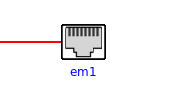
\includegraphics[width=0.15\textwidth]{./images/rj45_canvas.png}
  \caption{\emph{External interface node label}}
  \label{fig:rj45_canvas}
\end{figure}

Check that \emph{roadwarrior-router} has a properly configured IP address on
the network interface connected to the physical interface. Additionally, check
that routes which route packets between virtual network and the external
network through the physical interface exist in both the external network and
in the virtual network (on \emph{roadwarrior-router}).

Save this configuration to a new file by selecting the \emph{Save as} option
from the \emph{File} menu. Name the file \texttt{extended-topology.imn}.

\subsection{Attaching to a running experiment}
IMUNES gives you the possibility to run multiple independent experiments on one
physical computer. Therefore, we added the possibility of attaching to running
experiments through the IMUNES GUI. In the \emph{Experiment} menu, select the
option \emph{Attach to experiment}. A dialog similar to
\ref{fig:attach_to_experiment} is opened. Here you can select on which
experiment you would like to attach. You can attach to all experiments, those
that were started using batch mode and those that were executed from the GUI.
The window shows the following experiment parameters:

\begin{itemize}
\item Experiment ID
\item Filename of the topology
\item Time when the experiment was started.
\item Experiment screenshot (only if it was started through the GUI)
\end{itemize}

To attach to the you can double-click it's entry or use the \emph{Resume selected
experiment} button.
\begin{figure}[H]
  \centering
  \vspace{10pt}
  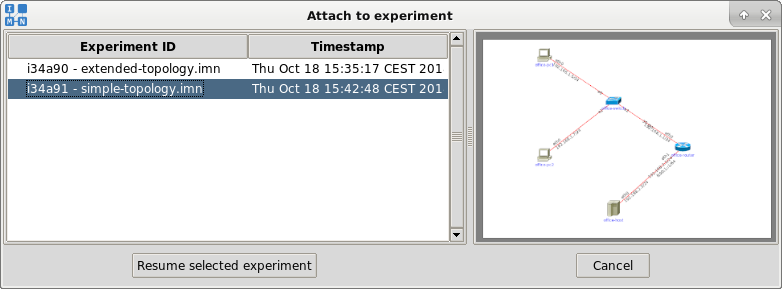
\includegraphics[width=0.90\textwidth]{./images/attach_to_experiment.png}
  \caption{\emph{Attach to experiment window}}
  \label{fig:attach_to_experiment}
\end{figure}
 
\section{Additional Configuration}

\subsection{Custom configuration}

%The configuration window of each network layer node (PC, host and router) also has the \emph{Custom startup configuration} field. The current startup
%configuration is generated with the \emph{Generate} button. In order to view or
%edit the generated startup configuration click on the \emph{Edit} button. In
%case of a PC, host or router with the static routing model, the default
%configuration consists of \emph{ifconfig} and \emph{route} commands.


The configuration window of each network layer node (PC, Host, Router, NAT64
and Click router) also has the \emph{Custom startup configuration} field. In
order to view or edit the generated startup configuration click on the
\emph{Editor} button as shown in Figure \ref{fig:config_tab}.

\begin{figure}[H]
\centering
\vspace{10pt}
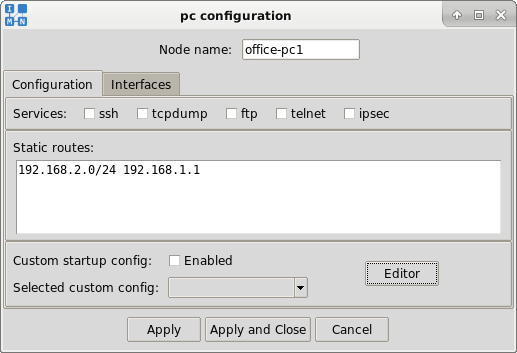
\includegraphics[width=0.6\textwidth]{./images/configuration_tab.png}
\caption{\emph{Configuration tab}}
\label{fig:config_tab}
\end{figure} 

In a newly opened window, write a new configuration name and click
\emph{Create}. An empty configuration file will be created. By clicking on
\emph{Fill defaults}, in case of a non-router network layer node or a router
node with the static routing model, the default configuration consists of
\emph{ifconfig} and \emph{route} commands with the \texttt{/bin/sh} shell.
Figure \ref{fig:custom_config} shows the created default configuration.

\begin{figure}[H]
\centering
\vspace{10pt}
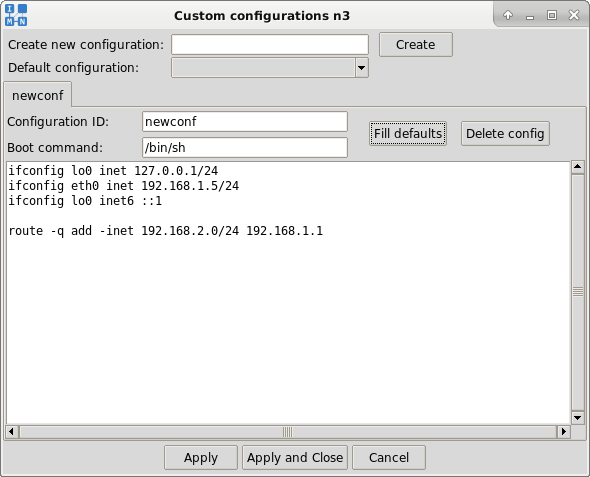
\includegraphics[width=0.6\textwidth]{./images/custom_configuration.png}
\caption{\emph{Custom configuration window}}
\label{fig:custom_config}
\end{figure}

It is possible to add custom commands that will be executed at the boot time.
When finished, click on the \emph{Apply} or \emph{Apply and Close} button to
save the changes. When you have multiple configurations, you can choose the
default one in the \emph{Default configuration} drop-down menu. To delete a
configuration, select its tab and click \emph{Delete config} button.

\textbf{NOTE:} After starting the network simulation, the new/custom
configuration will be considered only if \emph{Custom startup configuration} is
enabled. This is done by checking the \emph{Enabled} check box in the
\emph{Custom startup config} field in Figure \ref{fig:config_tab}.

\subsection{Physical and logical interfaces}

When the Interfaces tab is opened, a configuration window similar to the one
shown in Figure \ref{fig:phys_log_ifc} is shown to the user. The Physical
Interfaces list represents actual interfaces connected to links in IMUNES. Thus
we can see that the selected node has one link in IMUNES.

IMUNES also offers the feature to configure additional logical interfaces. By
default only one logical interface is added: \texttt{lo0} - the loopback
interface with the following addresses: \texttt{127.0.0.1} for IPv4 and
\texttt{::1} for IPv6. 

\begin{figure}[H]
\centering
\vspace{10pt}
\includegraphics[width=0.6\textwidth]{./images/physical_logical_interfaces.png}
\caption{\emph{Physical and logical interfaces}}
\label{fig:phys_log_ifc}
\end{figure} 

Users can configure additional logical interfaces by clicking on the Logical
Interfaces item in the Interfaces list. The Logical Interfaces configuration
window is show in Figure \ref{fig:logical_ifcs}.  At the moment IMUNES supports
two types of logical interfaces: \texttt{lo} and \texttt{vlan}.

\begin{figure}[H]
\centering
\vspace{10pt}
\includegraphics[width=0.6\textwidth]{./images/logical_interfaces.png}
\caption{\emph{Logical interfaces management}}
\label{fig:logical_ifcs}
\end{figure}

Figure \ref{fig:vlan_logical_ifcs} shows an example for setting up a
\texttt{vlan} logical interface \texttt{vlan0} on a physical interface
\texttt{eth0} with an arbitrary tag \texttt{10} and an IPv4 address
\texttt{10.0.0.1/24}.

\begin{figure}[H]
\centering
\vspace{10pt}
\includegraphics[width=0.6\textwidth]{./images/vlan_logical_interfaces.png}
\caption{\emph{Logical interfaces management}}
\label{fig:vlan_logical_ifcs}
\end{figure}

%\subsection{IPsec configuration}
%
%In the configuration window of the network layer elements (router, host and PC)
%you can also configure parameters referring  to the IPsec protocol. When you
%open the configuration window, beside other tabs, you'll see the \emph{IPsec}
%tab (Figure \ref{fig:IPsec}). With the \emph{Add SA/SP} button you can add a
%new \emph{Security Association/Security Policy}. You can also edit an existing
%SA/SP by selecting it from the list of saved SAs/SPs.
%\begin{figure}[H]
%\centering
%\vspace{10pt}
%\includegraphics[width=0.6\textwidth]{./images/IPsec.png}
%\caption{\emph{IPsec configuration}}
%\label{fig:IPsec}
%\end{figure} 
%Through this dialog only manual IPsec configuration is possible. It is disabled
%by default. All IPsec configuration parameters are written to the setkey.conf
%file. If there happen to be some syntax errors in the \emph{setkey.conf} file,
%it will be shown in the error window after starting the experiment.
%For an automated configuration it is possible to start the daemon named
%\emph{racoon} using a script and the \emph{himage} command.


\section{Additional Tools}
\subsection{Splitting a link}
Links can be split in two separate parts and it is possible to change location
of both of its parts after selecting it with the \emph{Select tool}. Right
click on the link and than left click on the \emph{Split label} in the pop-up
menu to split the link in two halves. Separated link parts can be merged back
with the \emph{Merge} option from the link menu. This feature is shown in
Figure \ref{fig:split_link}.

\begin{figure}[H]
\centering
\vspace{10pt}
\includegraphics[width=0.7\textwidth]{./images/split_link.png}
\caption{\emph{Split link}}
\label{fig:split_link}
\end{figure}

\subsection{Generating a network topology}
\label{sec:GeneratingNetworkTopology}
\emph{TopoGen} menu from the menubar enables easier and faster generation of
network topologies (Figure \ref{fig:topogen_menu_star}). This function can be
used to generate following topologies: \emph{Chain, Star, Cycle, Wheel, Cube,
Clique, Bipartite} or \emph{Random}. 

\begin{figure}[H]
\centering
\vspace{10pt}
\includegraphics[width=0.18\textwidth]{./images/topogen_menu_star.png}
\caption{\emph{TopoGen menu}}
\label{fig:topogen_menu_star}
\end{figure}

Some examples can be seen in Figure \ref{fig:star}, Figure \ref{fig:bipartite}
and Figure \ref{fig:wheel}. In order to generate a topology first select the
network layer nodes (router, host or PC) from the toolbox and then the desired
topology type e.g. bipartite graph K(2,3) (see Figure \ref{fig:bipartite}).

\begin{figure}[H]
\centering
\vspace{10pt}
\includegraphics[width=\textwidth]{./images/star.png}
\caption{\emph{Star topology}}
\label{fig:star}
\end{figure}

\begin{figure}[H]
\centering
% \vspace{10pt}
\includegraphics[width=\textwidth]{./images/bipartite.png}
\caption{\emph{Bipartite topology}}
\label{fig:bipartite}
\end{figure}

\begin{figure}[H]
\centering
% \vspace{10pt}
\includegraphics[width=\textwidth]{./images/wheel.png}
\caption{\emph{Wheel topology}}
\label{fig:wheel}
\end{figure}  

In case of \emph{random} topology an additional information is needed, so
beside the number of the nodes it is also necessary to specify the number of
links. The nodes in the random topology will be randomly connected with the
number of links specified before. An example of generating a \emph{random}
topology: 
  \begin{enumerate}
  \item Select the router tool from the toolbox.
  \item Choose the random topology: \emph{TopoGen $\to$ Random}
  \item Choose the desired number of nodes and links e.g. n = 6; m = 5, where n
is the number of nodes and  m  the number of links in the generated network
topology (\emph{Random $\to$ R(6,m) $\to$ R(6,5)}). 
 \end{enumerate}
 The result is shown in Figure \ref{fig:random}. 
 
\begin{figure}[H]
\centering
\vspace{10pt}
\includegraphics[width=\textwidth]{./images/random.png}
\caption{\emph{Random topology}}
\label{fig:random}
\end{figure} 
 
Using the \emph{TopoGen} tool you can generate topologies containing one type
of node (router, host or PC). In that case, new nodes of the same type are
created and placed on the canvas. Another option is to add new nodes to canvas
and then connect them using the topology generator:
\begin{enumerate}
  \item Add nodes to the canvas (don't have to be same type). 
  \item Select nodes that should be included in the new topology
  \item Right click on one of the selected nodes and choose the option
\emph{Create Link to} from the menu. Choose the option \emph{Selected} and
select one of the offered topologies (\emph{Chain, Star, Cycle, Clique} or
\emph{Random}). An example is shown in Figure \ref{fig:connect}. 
\end{enumerate}

In addition to that, it is also possible to transform existing nodes:
\begin{enumerate}
  \item Select nodes that should be transformed
  \item Right click on one of the selected nodes and choose the option
\emph{Transform to} from the menu. Select one of the offered options
(\emph{Router, PC} or \emph{Host}). An example is shown in Figure
\ref{fig:transform}.
\end{enumerate}

\begin{figure}[H]
\centering
\vspace{10pt}
\includegraphics[width=\textwidth]{./images/connect_1connect_2.png}
\caption{\emph{Example of creating a network topology with existing nodes}}
\label{fig:connect}
\end{figure}

\begin{figure}[H]
\centering
\vspace{10pt}
\includegraphics[width=\textwidth]{./images/transform.png}
\caption{\emph{Example of transforming existing network layer nodes}}
\label{fig:transform}
\end{figure}

\subsection{IPv4 address pool}
\label{sec:IPv4AddressPool}
\emph{IPv4 address pool} option from the \emph{Tools} menu is used for
replacing default 10.0.0.0/24 address pool. Choosing that option invokes a
dialog shown in Figure \ref{fig:ipv4_addr_pool}.

\begin{figure}[H]
\centering
\vspace{10pt}
\includegraphics[width=0.35\textwidth]{./images/ipv4_addr_pool.png}
\caption{\emph{IPv4 address pool dialog}}
\label{fig:ipv4_addr_pool}
\end{figure}

In order to replace default 10.0.0.0/24 address pool, set variable-mask IPv4
address pool through the invoked dialog. CIDR notation is required, so the IPv4
address needs to be followed by a slash and a network length. To apply changes
click on the \emph{Apply} button. The given address pool will be applied to all
the subsequentially created network layer elements (Figure
\ref{fig:ipv4_addr_pool_example}).

\begin{figure}[H]
\centering
\vspace{10pt}
\includegraphics[width=\textwidth]{./images/ipv4_addr_pool_example.png}
\caption{\emph{IPv4 address pool example}}
\label{fig:ipv4_addr_pool_example}
\end{figure}

In order to apply the given address pool to selected elements, right click on
the network layer element and choose the option \emph{IPv4 autorenumber} from
the popped up menu. In example shown in Figure
\ref{fig:ipv4_autorenumber_example} we have set IPv4 address pool to
160.153.1.1/24, selected all network elements and selected the option
\emph{IPv4 autorenumber} from the node menu to apply the given address pool to
selected elements.

\begin{figure}[H]
\centering
\vspace{10pt}
\includegraphics[width=\textwidth]{./images/ipv4_autorenumber_example.png}
\caption{\emph{IPv4 autorenumber example}}
\label{fig:ipv4_autorenumber_example}
\end{figure}

\subsection{IPv6 address pool}
\label{sec:IPv6AddressPool}
\emph{IPv6 address pool} option from the \emph{Tools} menu is used for
replacing default fc00::/64 address pool.
The procedure for setting the IPv6 address pool is the same as for setting the IPv4 address pool.

\subsection{Routing protocol defaults}
\label{sec:RoutingProtocolDefaults}
In the \emph{Tools} menu you can find the \emph{Routing protocol defaults}
option. Selecting this option invokes a popup window shown in Figure
\ref{fig:router_def_1}. Just as a reminder, settings referring to routing
protocols can be also changed in the \emph{router configuration} window. The
difference is that changes made there are applied only to the router that is
being configured. This tool in contrary makes it possible to apply changes to
one or more selected routers. If there is no router selected than the changes
will be applied to subsequentially created routers. Note that this option will
be disabled when the experiment starts.

\begin{figure}[H]
\centering
\vspace{10pt}
\includegraphics[width=0.35\textwidth]{./images/router_defaults_1.png}
\caption{\emph{Router defaults window}}
\label{fig:router_def_1}
\end{figure}

\section{Customizing Look}
\subsection{Annotations}
To emphasize some parts of the network topology, you can add various graphic
elements to the canvas. These elements are divided into three groups:
\begin{itemize}
    \item Text
    \item Freeform
    \item Oval
    \item Rectangle
\end{itemize}
Each of these elements have their own tools in the toolbox: \emph{Text} tool
(Figure \ref{fig:text}), \emph{Freeform} tool (Figure \ref{fig:freeform}),
\emph{Oval} tool (Figure \ref{fig:oval}) and \emph{Rectangle} tool (Figure
\ref{fig:rectangle}).

\begin{figure}[H]
  \centering
  \vspace{10pt}
  \includegraphics[width=0.07\textwidth]{./images/text_tool.png}
  \caption{\emph{Text tool}}
  \label{fig:text}
\end{figure}

\begin{figure}[H]
  \centering
  \vspace{10pt}
  \includegraphics[width=0.07\textwidth]{./images/freeform_tool.png}
  \caption{\emph{Freeform tool}}
  \label{fig:freeform}
\end{figure}

\begin{figure}[H]
  \centering
  \vspace{10pt}
  \includegraphics[width=0.07\textwidth]{./images/oval_tool.png}
  \caption{\emph{Oval tool}}
  \label{fig:oval}
\end{figure}

\begin{figure}[H]
  \centering
  \vspace{10pt}
  \includegraphics[width=0.07\textwidth]{./images/rectangle_tool.png}
  \caption{\emph{Rectangle tool}}
  \label{fig:rectangle}
\end{figure}

To add an annotation to the canvas, select the appropriate tool and click (and
drag) where you want to add the annotation. A popup window will be shown. There
you can define how will the annotation look.

When created, annotations can be moved around on the canvas. This is done by
using the select tool. Click on the annotation and then drag it to its
destination.

\subsubsection{Text}
The text annotation lets you define the following options(Figure
\ref{fig:text_conf}):
\begin{itemize}
    \item \emph{Text color} - color of the text in RGB values
    \item \emph{Font} - which system font, size and style you want to use
\end{itemize}

\begin{figure}[H]
	\centering
	\vspace{10pt}
	\includegraphics[width=0.55\textwidth]{./images/text_conf.png}
	\caption{\emph{Text configuration window}}
	\label{fig:text_conf}
\end{figure}

\subsubsection{Freeform}
The freeform configuration window includes:
\begin{itemize}
	\item \emph{Line color} - which line color to use
	\item \emph{Width} - line width to use
\end{itemize}

\begin{figure}[H]
	\centering
	\vspace{10pt}
	\includegraphics[width=0.30\textwidth]{./images/freeform_conf.png}
	\caption{\emph{Freeform configuration window}}
	\label{fig:freeform_conf}
\end{figure}

\subsubsection{Oval}
The size of the oval annotation is defined by dragging the cursor on the canvas
while keeping the left mouse button pressed. When the annotation size seems to
be fine, release the mouse button. The oval configuration window will popup
(Figure \ref{fig:oval_conf}).

The oval annotation lets you define the following additional options (Figure
\ref{fig:oval_conf}):
\begin{itemize}
    \item \emph{Fill color} - color of the annotation fill in RGB values.
    \item \emph{Border color} - color of the annotation border in RGB values.
    \item \emph{Border width} - width of the annotation border.
\end{itemize}

\begin{figure}[H]
	\centering
	\vspace{10pt}
	\includegraphics[width=0.55\textwidth]{./images/oval_conf.png}
	\caption{\emph{Oval configuration window}}
	\label{fig:oval_conf}
\end{figure}

\subsubsection{Rectangle}
The rectangle configuration window has the same options as the oval
configuration window. The rectangle size is defined the same way as the size of
the oval.

The rectangle annotation lets you define the following additional options
(Figure \ref{fig:rectangle_conf}):
\begin{itemize}
    \item \emph{Radius of the bend at the corners} - defines roundness of the
rectangle edges.
\end{itemize}

\begin{figure}[H]
	\centering
	\vspace{10pt}
	\includegraphics[width=0.55\textwidth]{./images/rectangle_conf.png}
	\caption{\emph{Rectangle configuration window}}
	\label{fig:rectangle_conf}
\end{figure}

Example of the annotations usage is shown in Figure \ref{fig:annotations_example}.

\begin{figure}[H]
	\centering
	\vspace{10pt}
	\includegraphics[width=\textwidth]{./images/annotations_example.png}
	\caption{\emph{Annotations example}}
	\label{fig:annotations_example}
\end{figure}

\subsection{Canvas background image}
\label{sec:CanvasBackgroundImage}

The options for changing the canvas background image are accessible through the
\emph{Canvas} and \emph{View} menu and through the menu that is opened with a
right click on the empty canvas (Figure \ref{fig:canvas_menu} and Figure
\ref{fig:background_image_menu}).

\begin{figure}[H]
	\centering
	\vspace{10pt}
	\includegraphics[width=0.4\textwidth]{./images/background_image_menu.png}
	\caption{\emph{Background image menu}}
	\label{fig:background_image_menu}
\end{figure}

All options related to the canvas background are accessible in the
\emph{Background image} menu (Figure \ref{fig:background_image_menu}):
\begin{itemize}
    \item \emph{Show background} - Show or hide the canvas background.
    \item \emph{Change background} - Opens the \emph{Change canvas background}
window (Figure \ref{fig:change_canvas_background}).
    \item \emph{Remove background} - Removes the background from the current
canvas.
    \item \emph{Set background from} - Sets the background from an another
canvas.
\end{itemize}

To set a canvas background you need to open the \emph{Change canvas background}
window (Figure \ref{fig:change_canvas_background}).

\begin{figure}[H]
	\centering
	\vspace{10pt}
	\includegraphics[width=0.75\textwidth]{./images/change_canvas_background.png}
	\caption{\emph{Change canvas background}}
	\label{fig:change_canvas_background}
\end{figure}

This window is divided into two main parts:
\begin{itemize}
    \item Left pane with the canvas background options
    \begin{itemize}
	\item Field and button for choosing the background image
	\item Image setting options
	\item Image alignment options
	\item Additional information if imagemagick is not present (Figure
\ref{fig:imagemagick_warning})
    \end{itemize}
    \item Right pane with canvas and image information and preview
    \begin{itemize}
	\item Canvas size information
	\item Image preview
	\item Image size information
    \end{itemize}
\end{itemize}

\begin{figure}[H]
	\centering
	\vspace{10pt}
	\includegraphics[width=0.78\textwidth]{./images/imagemagick_warning.png}
	\caption{\emph{Warning if ImageMagick is not present}}
	\label{fig:imagemagick_warning}
\end{figure}


When the image is selected there are four image setting modes that can be chosen:
\begin{itemize}
    \item \emph{Use original/cropped image} - If the image is smaller it will
be placed in the position defined by the image alignment. If the image is
larger  it will be cropped. The image alignment will define which part of the
image will be taken as the background.
    \item \emph{Stretch/shrink image} - If the image is smaller it will be
stretched without changing the proportions. If the image is larger it will be
shrunk without changing the proportions. The image alignment will define which
part of the image will be taken as the background.
    \item \emph{Adjust canvas to image} - The canvas will be resized to the
image size and then the background image will be set.
    \item \emph{Adjust image to canvas} - The image will be forcibly resized to
the canvas size with changed proportions if needed.
\end{itemize}

\subsubsection{Settings canvas background images}

We will use the extended topology example (\emph{extended-topology.imn}) to set
canvas background images. On the \emph{office-canvas} we will set a background
image. Then we will go to the \emph{roadwarrior-canvas} and set that same image
using the \emph{Set background from $\to$ office-canvas} option (Figure
\ref{fig:set_background_from}).

\begin{figure}[H]
	\centering
	\vspace{10pt}
	\includegraphics[width=0.4\textwidth]{./images/set_background_from.png}
	\caption{\emph{Set background from menu}}
	\label{fig:set_background_from}
\end{figure}

The final result is shown in Figure \ref{fig:canvas_background_example_1} and
Figure \ref{fig:canvas_background_example_2}.

\begin{figure}[H]
	\centering
% 	\vspace{10pt}
	\includegraphics[width=\textwidth]{./images/canvas_background_example_1.png}
	\caption{\emph{Canvas background example on office-canvas}}
	\label{fig:canvas_background_example_1}
\end{figure}

\begin{figure}[H]
	\centering
% 	\vspace{10pt}
	\includegraphics[width=\textwidth]{./images/canvas_background_example_2.png}
	\caption{\emph{Canvas background example on roadwarrior-canvas}}
	\label{fig:canvas_background_example_2}
\end{figure}

\subsection{Icons}
\label{sec:Icons}
IMUNES lets you choose custom node icons. First, select the nodes whose icons
you want to change. Then right click on the selection and then go to the
\emph{Node icon $\to$ Change node icons} option (Figure
\ref{fig:node_icon_menu}). This menu has also the \emph{Set default icons}
option that sets the default node icon for the selected icons.

\begin{figure}[H]
	\centering
	\vspace{10pt}
	\includegraphics[width=0.5\textwidth]{./images/node_icon_menu.png}
	\caption{\emph{Node icon menu}}
	\label{fig:node_icon_menu}
\end{figure}

The \emph{Change node icons} option opens the \emph{Set custom icon} window
(Figure \ref{fig:set_custom_icon}).

\begin{figure}[H]
	\centering
	\vspace{10pt}
	\includegraphics[width=0.6\textwidth]{./images/set_custom_icon.png}
	\caption{\emph{Set custom icon}}
	\label{fig:set_custom_icon}
\end{figure}

This window is divided into two main parts (Figure \ref{fig:set_custom_icon}):
\begin{itemize}
    \item Left pane for choosing custom icons
    \begin{itemize}
	\item List of library and custom icons on the top. Every icon that has
been used or is being used in the project will be available at the end of the
list, and will be given a generic name (e.g. img0, img5).
	\item Field and button for choosing the custom icon
    \end{itemize}
    \item Right pane with the icon preview and icon size information
\end{itemize}

We will now open the \emph{extended-topology.imn} file and set a custom icon.
We will choose the library icon \emph{ipfirewall.gif} for the
\emph{roadwarrior-router}. The final result is shown on Figure
\ref{fig:changed_node_icon}.

\begin{figure}[H]
	\centering
	\vspace{10pt}
	\includegraphics[width=\textwidth]{./images/changed_node_icon.png}
	\caption{\emph{Changed roadwarrior-router icon}}
	\label{fig:changed_node_icon}
\end{figure}

\subsubsection{Icon size}
If you want to emphasize the information about nodes, interfaces and links
instead of node icons you can change the icon size through the \emph{View $\to$
Icon size} option (Figure \ref{fig:icon_size}).
\begin{figure}[H]
	\centering
	\vspace{10pt}
	\includegraphics[width=0.4\textwidth]{./images/icon_size.png}
	\caption{\emph{Icon size menu}}
	\label{fig:icon_size}
\end{figure}

Let's take the \texttt{simple-topology.imn} example and set the icon size to
small. (Figure \ref{fig:icon_size_example})

Currently, only two sizes are available, normal and small. Otherwise, custom
icons can be used.

\begin{figure}[H]
	\centering
	\vspace{10pt}
	\includegraphics[width=\textwidth]{./images/icon_size_example.png}
	\caption{\emph{Icon size example}}
	\label{fig:icon_size_example}
\end{figure}

\section{User-configurable Event Scheduling}
\label{sec:using event scheduler}
This section describes a feature for scheduling of arbitrary deterministic and
stochastic events during experiment execution.

\subsection{Principle of operation}
The control plane in IMUNES is extended to retain control over the experiment
execution after initial topology instantiation, allowing for user-scheduled
events to influence selected parameters during run time.

The current implementation allows for the event scheduler to assume control
over selected link properties such as:
\begin{itemize}
\item bandwidth
\item delay
\item bit error rate
\item packet duplication
\item visual attributes
\begin{itemize}
\item line width
\item line color
\end{itemize}
\end{itemize}

The event scheduler supports two general classes of schedulable events:
one-time changes and periodic functions. 

One-time events update the selected parameter at requested point in time,
leaving that parameter constant throughout rest of the experiment execution, or
until another event updates it to a new value at some later point in time. 

Periodic functions allow for time-variant functions to be applied to selected
parameters by specifying those functions as single events. Subsequently
scheduled events acting upon the same parameter will cancel the current
periodic function and replace it with either a constant value or another
periodic function.

\subsection{Configuring events with events editor}
Events can be specified in the \emph{Events editor} (Figure
\ref{fig:event_editor}). To open the \emph{Events editor} select the
\emph{Events} $\to$ \emph{Events editor} option. The editor is divided into two
elements. The left side element contains a list of all links. The right side
element contains events configured on the selected link. This dialog allows you
to edit events on that link. To save the event scheduling configuration you
need to click on \emph{Apply} button. The events editor gives you the
possibility to start or stop the event scheduling during experiment execution.
This can be also done from the \emph{Events} menu in the menubar.

\begin{figure}[H]
	\centering
	\vspace{10pt}
	\includegraphics[width=0.65\textwidth]{./images/event_editor.png}
	\caption{\emph{Events editor}}
	\label{fig:event_editor}
\end{figure}

Each event entry occupies a single line of text, consisting of four fields:
deadline, target parameter, function and function parameters. The first field,
deadline, is specified as an integer number of seconds since experiment
instantiation. The second field, target parameter, may be one of the following:
bandwidth, delay, ber, duplicate, width or color. The remainder of the line is
further parsed as a function. The type of the function is determined by the
leading keyword, which may be either const, ramp, rand or square. When saving
the configuration through the events editor a syntax check will be performed.
If the syntax is wrong the configuration will not be saved and a popup dialog
will show the first line that has a syntax error.

\subsubsection{Const}
The const function accepts one parameter, the target value. After the deadline
time the parameter will constantly be equal to the target value.

\subsubsection{Ramp}
Behavior of the ramp function is determined by three arguments: initial value,
delta, and period, which are all integers. The first argument represents the
initial function value. The second is the delta value, which may be both
positive or negative, which is added to the previous value of the function at
each period. The third argument is the period, determining how often will the
delta value be added to the current function value.

\subsubsection{Rand}
The rand function is determined by three arguments: lower bound, upper bound,
and period; all of which are integers. The function will assume a random value
between lower and upper bound after each period (in seconds) expires.

\subsubsection{Square}
Finally, the square function has three arguments as well: low value, high
value, and period; all integer numbers. The resulting function will flip from
low value to high and vice versa after each period (in second) expires.

\subsubsection{Example}
The following example illustrates a possible event scheduling scenario that can be entered in the Event editor window (Figure \ref{fig:event_editor}):

\begin{alltt}
    30 bandwidth ramp 128000 8000 2
    30 delay rand 80000 120000 8
    60 delay square 100000 200000 10
    60 ber const 1
    90 ber const 0
    120 delay const 0
\end{alltt}

At t = 30 s, bandwidth of the selected link will be set to 128 Kbps, and will
continue to grow at a rate of 8 Kbps each 2 s.

Also at t = 30 s, the delay will begin assuming a random value between 80 ms
and 120 ms, and will continue to change the setting to new random values in the
same range each 8 s.

At t = 60 s, the delay will cease to assume random values, and instead it will
begin to oscillate between two discrete values, 100 ms and 200ms, each 10 s.

Also at t = 60 s, the bit error rate (BER) will be set to 1, resulting in all
frames traversing the link to be silently dropped.

At t = 90 s, the BER is reset back to 0, allowing for all frames to traverse
the link without artificial losses.

At t = 120 s, the oscillation of the delay parameter will stop, and delay will
be reset to 0 ms for the rest of the experiment execution time.

The current time is shown on the status bar after the zoom value. (Figure
\ref{fig:statusbar_execute})

\subsection{Configuring events through configuration file}
\textbf{NOTE:} It is advised to use the Events editor to configure event
scheduling because it includes a syntax check. In the case of configuring
events through configuration file, the wrong syntax will be silently ignored.

IMUNES experiments are defined via plain-text configuration files, which
currently describe virtual nodes and links, as well as additional objects
related only to GUI visual properties and annotations. The other way to
configure events is manual editing of an existing configuration file.

The example bellow shows a configuration section describing a virtual link in
an IMUNES experiment. The link l0 connects virtual nodes n0 and n1, has the
bandwidth constraint set to 128 Kbps, and has the thickness of the line
representing the link in the GUI set to 6 pixels. All of the mentioned
properties are directly controllable via the IMUNES GUI. The configuration for
link l0 also includes an empty placeholder for schedulable events, meaning that
no events have been programmed for this link.

\begin{alltt}
link l0 \{
    width 6
    nodes \{n0 n1\}
    bandwidth 128000
    \emph{events \{}
    \emph{\}}
\}
\end{alltt}

The events section in the configuration file accepts the same commands as does
the Events editor in the GUI.


\section{Starting and terminating a simulation through CLI}
In addition to the \emph{File$\to$Open} option to open an .imn file and the
\emph{Experiment$\to$Execute} option used to initiate the virtual network
topology in the GUI, the simulation can be initiated through the command-line
interface (CLI) with the following command:

\texttt{\# imunes -b simple-network.imn}
 
Using IMUNES through GUI, the \emph{Experiment$\to$Terminate} option is used
for shutting down the simulation and cleaning up the virtual network topology
from the kernel. The CLI alternative for the latter is the following command:

\texttt{\# imunes -b -e experimentId}

The parameter \texttt{exeperimentId} represents the experiment identifier. In
order to get the experiment identifier you can use the \texttt{himage} command.
With \texttt{himage -l} you will get a list of identifiers of all started
experiments. 

% In Figure \ref{fig:***} you can see the output for the line:
%  
% \texttt{\# vimage -l}
% 
% As you can see, there are two experiment identifiers listed, one is *** and
% the other is ***. In the next Figure \ref{fig:***} you can see the output for
% the line:
% 
% \texttt{\# vimage -lr}
% 
% In this output, beside the experment identifiers, you also get the list of
% network layer nodes with the information to which experiment they belong.
% This can be useful if you have more than one experiment started on your PC
% and can't resolve which identifier belongs to which experiment. With the
% additional information, which nodes the experiment conatains, it can be
% easier to distinguish the experiments.   

\section{Managing virtual nodes (jails) - jls, jexec}
The FreeBSD jail mechanism allows partitioning of a FreeBSD-based computer
system into several independent smaller systems called jails. This mechanism
enables creation of a safe environment, separate from the rest of the system.
Processes created inside a jail are limited within that jail environment. Each
jail is a virtual environment running on the host machine, having its own file
system, processes, set of users, networking subsystem of the FreeBSD kernel and
a few other things.     

Two main commands exist in FreeBSD for manging and configuring previously
created jails:
\begin{itemize}
\item \texttt{jexec} - executes a command inside an existing jail
\item \texttt{jls} - lists jails.
\end{itemize}

A virtual image or vimage is a jail with its own independent network stack
instance.  Every process, socket and network interface present in the system is
always attached to one, and only one, virtual network stack instance (vnet).
During system bootup sequence a default vnet is created to which all the
configured interfaces and user processes are initially attached. 

The \texttt{jexec} command allows for execution of arbitrary processes in a
targeted virtual image.

\texttt{jexec jname command ...} \hfill

The jexec command starts the selected command and it's arguments in the jail
\texttt{jname}.

To find out the names of started jails the jls command is used: 

\texttt{jls [-hnqsv] [parameter ...]} \hfill
 
Since the default jls command doesn't list names of jails a better output is
provided using the command:

\texttt{jls -h jid name host.hostname} \hfill

Also, the command \texttt{jls -v} gives a more detailed output.

\subsection{Examples}

Execute the \texttt{ifconfig} command in the jail with the jail name
\texttt{n1}:

\texttt{\# jexec n1 ifconfig} \hfill

Execute the \texttt{csh} command in the IMUNES virtual node named \texttt{host1}:

First we need to find out the jail ID or jail name to execute the wanted
command:

\texttt{\# jls -h jid name host.hostname | grep host1} \hfill

The first parameter output is the jail ID, the second is the jail name and the
last is the hostname. To execute the command you need the jail ID or jail name:

\texttt{\# jexec \emph{jid} csh} \hfill

\texttt{\# jexec \emph{jname} csh} \hfill

\section{Himage tool}
The jls and jexec commands can be impractical for creating scripts for
topologies since the output of the jls command is needed for starting the jexec
command. The jexec command can't take the hostname of the jail as an argument,
it can only take the jail name or jail id. The jail name is created from the
IMUNES experiment ID and the node identifier (not hostname). Every experiment
started in IMUNES has a different randomly generated experiment ID to enable
execution of multiple experiments at once.

IMUNES comes with the \texttt{himage} tool that enables the usage of hostnames
when starting commands in virtual nodes. The \texttt{himage} tool starts the
jexec command with the appropriate jail name so that the user doesn't have to
search for it. 

The \texttt{himage} command has the following options:
\begin{itemize}
\item \texttt{himage vi\_hostname command ...} - executes the command in the virtual
node with the specified hostname. If no command is specified, it starts an
interactive shell.
\item \texttt{himage -m vi\_hostname} - executes the command in the experiment
master jail. If no command is specified, it starts an interactive shell.
\item \texttt{himage -v vi\_hostname} - gets the jail node name of the virtual
node with the specified hostname
\item \texttt{himage -n vi\_hostname} - gets the node identifier for the
specified hostname.
\item \texttt{himage -e vi\_hostname} - gets the experiment ID in which the virtual
node with the specified hostname is running.
\item \texttt{himage -j/-i vi\_hostname} - gets the jail ID in which the virtual
node with the specified hostname is running.
\item \texttt{himage -d} - gets the hostname jail filesystem path on the host
machine.
\item \texttt{himage -l} - gets the experiment list with the experiment data.
\item \texttt{himage -ln} - gets the experiment list with node names.
\end{itemize}

\subsection{Examples}

Example of usage of the command himage on a node with the hostname "pc" to get a
list of running processes:

\texttt{\# himage pc ps ax} \hfill

If there are multiple experiments running and there are nodes with the same
hostnames in these experiments the \texttt{himage} command accepts the following
node specification where \texttt{vi\_hostname} is specified as
\texttt{hostname@eid}, where eid is the experiments' ID.

\texttt{\# himage hostname@eid command ...} \hfill

i.e:

\texttt{\# himage pc@i3d05a ps ax} \hfill

where \texttt{i3d05a} is the experiment ID of the running experiments. To find
out which experiments are running the \texttt{himage -l} command can be used as
well as \texttt{jls -h jid name host.hostname}.

Execute the \texttt{ifconfig} command the IMUNES node named \texttt{server}:

\texttt{\# himage server ifconfig}

\section{Hcp tool}

While the \texttt{himage} command is used for running programs inside virtual
nodes the \texttt{hcp} is used to copy files directly to the filesystem of
running mobile nodes, thus simplifying deployment of configuration files for
starting various services on virtual nodes.

Usage of the command \texttt{hcp}:

\texttt{hcp [cp\_command\_options] [vi\_hostname1:]filename
[vi\_hostname2:]filename} \hfill

The \texttt{hcp} command invokes the cp command with the specified options. If
the \texttt{vi\_hostname1} is specified the script copies a file from the
virtual node, otherwise it copies a file from the local folders. The second
\texttt{vi\_hostname2} specifies on which node the first file will be copied, if
not specified the file is copied to the local folders.

\texttt{vi\_hostname} is specified in the same way as in the \texttt{himage}
command, \texttt{hostname} or \texttt{hostname@eid}.

\subsection{Examples}

Copy file dhcpd.conf from a local folder to the virtual node DHCP:

\texttt{\# hcp dhcpd.conf DHCP:/usr/local/etc/} \hfill

Copy file message.txt from the virtual node PC to a local folder:

\texttt{\# hcp PC:/root/message.txt .} \hfill

Copy file index.html from the virtual node HOST to the virtual node HTTP:

\texttt{\# hcp HOST:/usr/local/www/data/index.html HTTP:/usr/local/www/data/} \hfill

\section{Example (himage and hcp)}

This is an example of starting an DHCP server through a script with the
provided configuration file dhcpd.conf.

Kill the server if it's started:

\texttt{\# himage DHCP killall -9 dhcpd} \hfill

Copy the configuration file:

\texttt{\# hcp dhcpd.conf DHCP:/usr/local/etc/} \hfill

Create the \texttt{.leases} file defined in \texttt{dhcpd.conf}:

\texttt{\# himage DHCP touch /var/db/dhcpd.leases} \hfill

Start the sever with the copied configuration file:

\texttt{\# himage DHCP dhcpd -cf /usr/local/etc/dhcpd.conf} \hfill

\section{Vlink tool}

The \texttt{vlink} tool is used to change link parameters. The following link parameters are available:
\begin{itemize}
	\item bandwidth (bps, bits-per-second)
	\item bit-error rate, BER (number of bits in which one error will occur)
	\item delay (microseconds)
	\item packet duplication (\%, percentage of packets that will be duplicated)
\end{itemize}

A link is identified by the endpoint node names. The link between pc1 and pc2 is identified by \emph{pc1:pc2} or \emph{pc2:pc1}.

Usage of the command \texttt{vlink}:

\texttt{vlink [options] link\_name[@eid]} \hfill

\subsection{Examples}

Setting the bandwidth to 10 Mb/s with a delay of 30 ms to the link connecting \emph{router1} and \emph{pc1}:

\texttt{\# vlink -bw 10000000 -dly 30000 router1:pc1}

Generate an error on one bit in a million:

\texttt{\# vlink -BER 1000000 router1:pc1}

Set packet duplication to 20%:

\texttt{\# vlink -dup 20 router1:pc1}

Modifying a link in a specific experiment (i.e. Experiment ID = i56ad1):

\texttt{\# vlink -dup 20 router1:pc1@i56ad1}

To reset the link settings to the default values the -r flag is used:

\texttt{\# vlink -r router1:pc1@i56ad1}

Check all \texttt{vlink} arguments with:

\texttt{\# vlink -h}




   \appendix
   \chapter{Installation}

\section{Installation of IMUNES on FreeBSD 8}

\subsection{Installing FreeBSD}
A comprehensive and explanatory guide for installing configuring and using
FreeBSD can be found here:

\begin{center}
\url{http://www.freebsd.org/doc/handbook/}
\end{center}

Section 2 of the handbook describes the installation of the FreeBSD operating
system: 
\begin{center}
\url{http://www.freebsd.org/doc/handbook/install.html}
\end{center}

You can choose to install FreeBSD with two different architectures:
\begin{itemize}
\item i386 - 32-bit - works on most personal computers.
\item amd64 - 64-bit - works on newer computers that support 64-bit processing.
Adds support for more RAM.
\end{itemize}

\subsection{Step by step guide through the FreeBSD installation}
\begin{enumerate}
\item Insert the FreeBSD-8.2-RELEASE or FreeBSD-8.3-RELEASE (i386 or amd64) 
medium on startup. Boot from it.
\item Country Selection - Choose your country (e.g. United States). Press
OK.
\item Main Menu - Choose the "Standard" installation. Press Select.
\item Message - Press OK.
\item FDISK Partition Editor - Press C to create a slice:
    \begin{enumerate}
    \item A minimum of 20GB is needed for FreeBSD. Type 20G to create a 20GB
    slice. Press OK.
    \item A screen with the number 165 appears. Press OK.
    \item Position on the created partition (probably named \texttt{ad0s1}).
    \item Press S to set the created partition bootable.
    \end{enumerate}
\item FDISK Partition Editor - Position on the "unused" space beneath the
created partiton. Press C to create another slice:
    \begin{enumerate}
    \item A minimum of 5GB is needed for ZFS. Type 5G to create a 5GB slice. Press OK.
    \item A screen with the number 165 appears. Press OK.
    \item Remember the name of this partition (probably named \texttt{ad0s2}).
    This name will be later used for configuring ZFS.
    \end{enumerate}
\item FDISK Partition Editor - Press Q to finish.
\item Boot Manager - Select the "Standard" option. Press OK.
\item Message - Press OK.
\item FreeBSD Disklabel Editor - While the partition "ad0s1" (the 20GB one) is
selected press A to automatically distribute system partitions on it.
\item FreeBSD Disklabel Editor - The result should look similar to this:
    \begin{verbatim}
    Part      Mount     Size
    ad0s1a    /       1024MB
    ad0s1b    swap    2006MB
    ad0s1d    /var    5099MB
    ad0s1e    /tmp    1024MB
    ad0s1f    /usr   11326MB
    \end{verbatim}
\item FreeBSD Disklabel Editor - Press Q.
\item Choose Distributions - Select the "6 User" distribution.
\item FreeBSD Documentation Installation Menu - Select "en" and then "X Exit".
\item Ports collection installation - Select "Yes".
\item Choose Distributions - Select the "X Exit" to exit. Press OK.
\item Choose Installation Media - Select "1 CD/DVD Install from a FreeBSD CD/DVD".
\item Continue through the Installation - Select "Yes".
\item Wait until the installation is over.
\item Message - Press OK.
\item Configure any ethernet devices? - Select "Yes".
    \begin{enumerate}
    \item Select the wanted ethernet device, e.g. \texttt{em0}.
    \item IPv6 configuration - Select "No".
    \item DHCP configuration - Select "Yes".
    \item Enter the hostname, e.g. IMUNES1.
    \item Select "OK".
    \end{enumerate}
\item Network gateway - Select "No".
\item Install inetd services - Select "No".
\item Allow SSH login - Select "Yes".
\item Allow anonymous FTP access - Select "No".
\item NFS server - Select "No".
\item NFS client - Select "No".
\item Customize system console settings - Select "No".
\item Set time zone - Select "No".
\item Configure mouse - Select "No".
\item Browse package collection - Select "No".
\item Add additional user accounts - Select "No".
\item Message - Set root password - Press "OK". Enter password. Re-enter
password.
\item Visit the general configuration menu - Select "No".
\item Main Menu - Select the "X Exit Install" option by using the "Tab" key.
\item Are you sure you want to exit? - Select "Yes".
\item Message - Reboot - Press "OK".
\end{enumerate}

\subsection{Installing the FreeBSD X11 system - GUI}

Login into the machine as root. Edit the file \texttt{/etc/rc.conf} with an editor e.g.
\texttt{vi} and add the following lines at the end of the file:
\begin{verbatim}
hald_enable="YES"
dbus_enable="YES"
zfs_enable="YES"
\end{verbatim}
Save changes and exit.

\texttt{\# pkg\_add -r xorg bash xpdf vim geany zip unzip xterm firefox}

You can choose between multiple desktop environments:
\begin{itemize}
\item Gnome2-lite - complete, user-friendly desktop\\
\texttt{\# pkg\_add -r gnome2-lite}
\item XFCE 4 - lightweight desktop environment\\
\texttt{\# pkg\_add -r xfce4}
\item IceWM - extremely lightweight window manager, low resource usage\\
\texttt{\# pkg\_add -r icewm}
\end{itemize}

After the installation of one or multiple window manager we need to configure
which will be used. Edit the file \texttt{.xinitrc} in the user folder and add a line
depending on which window manager you want to use:
\begin{itemize}
\item Gnome2-lite\\
\texttt{exec gnome-session}
\item XFCE 4\\
\texttt{exec startxfce4}
\item IceWM\\
\texttt{exec icewm-session}
\end{itemize}

Reboot the machine by issuing the \texttt{reboot} command:\\
\texttt{\# reboot}

After the machine has rebooted, log in and issue the \texttt{startx} command to
start the chosen window manager:\\
\texttt{\# startx}

\subsection{Installing IMUNES}

First we need to install the packages needed for IMUNES. To do this execute the
following command:

\texttt{\# pkg\_add -r tk86 ImageMagick tcllib libimg wireshark}

After all the packages are installed we need to use the second partition we
prepared during the installation (the one with the size 5GB, probably named
\texttt{ad0s2}). This partition will be used to store the data that will be in
the virtual nodes. For this purpose we will create a ZFS pool on the second
partition with the command \texttt{zpool create} assuming that the second
partition is named \texttt{ad0s2}:

\texttt{\# zpool create vroot /dev/ad0s2}

Now we need to fetch the IMUNES source/tarball from the official imunes site:

\begin{center}
\url{http://imunes.tel.fer.hr/imunes-1.0.tar.gz}
\end{center}

To fetch you can use the firefox browser that we installed earlier or use the
\texttt{fetch} command:

\texttt{\# fetch http://imunes.tel.fer.hr/imunes-1.0.tar.gz}

To extract the tarball use the following command:

\texttt{\# tar xf imunes-1.0.tar.gz}

Enter the extracted directory:

\texttt{\# cd imunes}

Now we need to install IMUNES and populate the ZFS file system with predefined
and required data. To install imunes on the system execute:

\texttt{\# make install}

To setup the ZFS file system execute:

\texttt{\# make vroot}

Both of these commands can be executed together by executing:

\texttt{\# make}

Now the IMUNES GUI can be ran just by typing the \texttt{imunes} command in the
terminal:

\texttt{\# imunes}

The GUI allows the specification of network topologies but to execute
experiments the FreeBSD kernel must be compiled with a few additional options.

\subsection{Recompiling the FreeBSD kernel with VIMAGE support}

First, the kernel sources need to be fetched, this can be done by using the
sysinstall utility:
\begin{enumerate}
\item Start the sysinstall utility:\\
\texttt{\# sysinstall}
\item Go to "Configure".
\item Go to "Distributions".
\item Go to "sys".
\item Mark "src" by pressing the Space key on it.
\item Select "X Exit".
\item Select "X Exit".
\item Select "Install from an FTP server".
\item Choose the "Main server" or a server closer to your location.
\item When the installation is done select press the Esc key until you exit the
sysinstall utility.
\end{enumerate}

Now the kernel source is available in the folder \texttt{/usr/src/sys}. Enter
that folder:

\texttt{\# cd /usr/src/sys}

Depending which distribution architecture you have decided to install, i386 or
amd64 the next command differs.

For i386 enter the directory \texttt{i386/conf}:

\texttt{\# cd i386/conf}

For amd64 enter the directory \texttt{amd64/conf}:

\texttt{\# cd amd64/conf}

With an editor (vi, vim or geany) create a file named \texttt{VIMAGE}:

\texttt{\# vi VIMAGE}

Insert the following configuration in the \texttt{VIMAGE} file:

\texttt{include	GENERIC \\
nooptions   FLOWTABLE \\
options	    VIMAGE \\
options	    VNET\_DEBUG \\
options	    MROUTING \\
 \\
options	    DDB \\
options	    KDB \\
}

Exit and save the file.

Now execute the following commands:
\begin{verbatim}
# config VIMAGE
# cd ../compile/VIMAGE
# make cleandepend && make depend
# make
# make install
\end{verbatim}

When the last command ends use the \texttt{reboot} command to restart the
computer:

\texttt{\# reboot}

\subsection{Running IMUNES on FreeBSD}

After login execute the \texttt{startx} command to start the window manager.
Open a terminal and start imunes:

\texttt{\# imunes}

Now you can create an arbitrary network topology or something like shown in
Figure \ref{fig:simple_topology} and execute the experiment.

\section{Installation of IMUNES on FreeBSD 9}

\subsection{Installing FreeBSD}
A comprehensive and explanatory guide for installing configuring and using
FreeBSD can be found here:

\begin{center}
\url{http://www.freebsd.org/doc/handbook/}
\end{center}

Section 2 of the handbook describes the installation of the FreeBSD operating
system: 
\begin{center}
\url{http://www.freebsd.org/doc/handbook/bsdinstall-start.html}
\end{center}

You can choose to install FreeBSD with two different architectures:
\begin{itemize}
\item i386 - 32-bit - works on most personal computers.
\item amd64 - 64-bit - works on newer computers that support 64-bit processing.
Adds support for more RAM.
\end{itemize}

\subsection{Step by step guide through the FreeBSD installation}
\begin{enumerate}
\item Insert the FreeBSD-9.2-RELEASE or FreeBSD-9.3-RELEASE (i386 or amd64) medium on startup. Boot from it.
\item Welcome - Choose "Install".
\item Keymap Selection
	\begin{enumerate}
		\item FreeBSD 9.3 - Press "Select" to "Continue with default keymap" or choose an alternative one.
		\item FreeBSD 9.2 - If you use a non-default key mapping for your keyboard, choose "Yes" and find your keyboard. Otherwise, choose "No".
	\end{enumerate}
\item Set Hostname - Set the hostname for your newly installed system (e.g. "imunes").
\item Distribution Select - Select "src" and "lib32" (only on amd64 architecture) and deselect "games" and "ports".
\item Partitioning - choose Guided or Manual
	\begin{itemize}
	\item Guided - Choose a disk from the list (e.g. "ada0"). Select "Entire Disk". In the Confirmation window choose "Yes" to erase the entire disk. In the "Partition Editor" review the changes. 	After finishing partitioning, choose "Finish" and then "Commit".
	\item Manual - example for manual partitioning for a 40GB slice:
	    \begin{verbatim}
	    Part        Type            Mount   Size
	    ada0p1      freebsd-boot            64kB
	    ada0p2      freebsd-ufs     /        2GB
	    ada0p3      freebsd-ufs     /var     8GB
	    ada0p4      freebsd-ufs     /tmp     4GB
	    ada0p5      freebsd-ufs     /usr    24GB
	    ada0p6      freebsd-swap    none     2GB
	    \end{verbatim}
	\end{itemize}
	After finishing partitioning, choose "Finish" and then "Commit".
NOTE: freebsd-boot boot partition will be created upon creation of the first freebsd-ufs partition.
\item Archive extraction - Wait for the installation to complete.
\item FreeBSD Installer - Enter your system administrator (root) password. Repeat the password.
\item Network Configuration - Choose a network interface to configure (if any available).
	\begin{enumerate}
	\item Select "Yes" to configure IPv4 network if you use it. Then select "Yes" to configure DHCP if you use it.
	\item Select "Yes" to configure IPv6 network if you use it. Then select "Yes" to configure SLAAC if you use it.
	\item Resolver Configuration - If DHCP/SLAAC is used to configure the interface, some values may already be present. Otherwise, enter them yourself.
	\end{enumerate}
\item Timezones - If your timezone is not UTC, select "No" and choose your region and country (e.g. Europe->Croatia) and select "Yes" if asked for confirmation.
\item System Configuration
	\begin{enumerate}
		\item FreeBSD 9.3 - Choose the "sshd" service to be started at boot and select "dumpdev" to enable crash dumps in /var.
		\item FreeBSD 9.2 - Choose the "sshd" service to be started at boot.
	\end{enumerate}
\item (FreeBSD 9.2 only) Dumpdev Configuration - Select "Yes" for enabling crash dumps in /var folder.
\item Add User Accounts - If necessary, add additional users now.
\item Final Configuration - Choose "Exit".
\item Manual Configuration - Nothing else is needed, so choose "No" to skip manual configuration.
\item Complete - Reboot. (Don't forget to remove your FreeBSD boot media.)
\end{enumerate}

\subsection{Installing the FreeBSD X11 system - GUI}

Login into the machine as root. Edit the file \texttt{/etc/rc.conf} with an editor e.g.
\texttt{vi} and add the following lines at the end of the file:
\begin{verbatim}
hald_enable="YES"
dbus_enable="YES"
\end{verbatim}
Save changes and exit.

\texttt{\# pkg\_add -r xorg bash xpdf vim geany zip unzip xterm firefox subversion}

You can choose between multiple desktop environments:
\begin{itemize}
\item Gnome2-lite - complete, user-friendly desktop\\
\texttt{\# pkg\_add -r gnome2-lite}
\item XFCE 4 - lightweight desktop environment\\
\texttt{\# pkg\_add -r xfce4}
\item IceWM - extremely lightweight window manager, low resource usage\\
\texttt{\# pkg\_add -r icewm}
\end{itemize}

After the installation of one or multiple window manager we need to configure
which will be used. Edit the file \texttt{.xinitrc} in the user folder and add a line
depending on which window manager you want to use:
\begin{itemize}
\item Gnome2-lite\\
\texttt{exec gnome-session}
\item XFCE 4\\
\texttt{exec startxfce4}
\item IceWM\\
\texttt{exec icewm-session}
\end{itemize}

Reboot the machine by issuing the \texttt{reboot} command:\\
\texttt{\# reboot}

After the machine has rebooted, log in and issue the \texttt{startx} command to
start the chosen window manager:\\
\texttt{\# startx}

\subsection{Installing IMUNES}

First we need to install the packages needed for IMUNES. To do this execute the
following command:

\texttt{\# pkg\_add -r tk86 ImageMagick tcllib wireshark socat gmake}

Now we need to fetch the IMUNES source/tarball from the official imunes site:

\begin{center}
\url{http://imunes.tel.fer.hr/imunes-1.0.tar.gz}
\end{center}

To fetch you can use the firefox browser that we installed earlier or use the
\texttt{fetch} command. Then extract the tarball and enter the directory:

\texttt{\# fetch http://imunes.tel.fer.hr/imunes-1.0.tar.gz}\\
\texttt{\# tar xf imunes-1.0.tar.gz}\\
\texttt{\# cd imunes\_\emph{version}}

Alternatively, you could checkout the last fresh IMUNES source through the
public SVN repository:

\texttt{\# svn co svn://imunes.tel.fer.hr/head/ imunes}\\
\texttt{\# cd imunes}

Now we need to install IMUNES and populate the virtual file system with predefined and required data. To install imunes on the system execute:

\texttt{\# make install}

To setup the virtual file system execute:

\texttt{\# make vroot}

Both of these commands can be executed together by executing:

\texttt{\# make}

Now the IMUNES GUI can be ran just by typing the \texttt{imunes} command in the
terminal:

\texttt{\# imunes}

The GUI allows the specification of network topologies but to execute
experiments the FreeBSD kernel must be compiled with a few additional options.

\subsection{Recompiling the FreeBSD kernel with VIMAGE support}

If you didn't include the src option in step 4 while installing FreeBSD, the
kernel sources need to be fetched. Use your selected architecture and release combination:

\texttt{\# fetch ftp://ftp.freebsd.org/pub/FreeBSD/releases/\emph{arch}/\emph{release}/src.txz}

e.g. for FreeBSD 9.2 with amd64 architecture use:

\texttt{\# fetch ftp://ftp.freebsd.org/pub/FreeBSD/releases/amd64/9.2-RELEASE/src.txz}

Extract it by using:

\texttt{\# tar xf src.txz -C /}

Now the kernel source is available in the folder \texttt{/usr/src/sys}. Enter
that folder:

\texttt{\# cd /usr/src/sys}

Depending which distribution architecture you have decided to install, i386 or
amd64 the next command differs.

For i386 enter the directory \texttt{i386/conf}:

\texttt{\# cd i386/conf}

For amd64 enter the directory \texttt{amd64/conf}:

\texttt{\# cd amd64/conf}

With an editor (vi, vim or geany) create a file named \texttt{VIMAGE}:

\texttt{\# vi VIMAGE}

Insert the following configuration in the \texttt{VIMAGE} file:

\texttt{include	GENERIC \\
nooptions FLOWTABLE \\
options VIMAGE \\
options VNET\_DEBUG \\
options MROUTING \\
 \\
options IPSEC \\
device crypto \\
options IPSEC\_DEBUG \\
 \\
options DDB \\
options KDB \\
}

Exit and save the file.

Now execute the following commands:
\begin{verbatim}
# config VIMAGE
# cd ../compile/VIMAGE
# make cleandepend && make depend
# make
# make install
\end{verbatim}

When the last command ends use the \texttt{reboot} command to restart the
computer:

\texttt{\# reboot}

\subsection{Running IMUNES on FreeBSD}

After login execute the \texttt{startx} command to start the window manager.
Open a terminal and start imunes:

\texttt{\# imunes}

Now you can create an arbitrary network topology or something like shown in
Figure \ref{fig:simple_topology} and execute the experiment.

\section{Installation of IMUNES on FreeBSD 10}

\subsection{Installing FreeBSD}
A comprehensive and explanatory guide for installing configuring and using
FreeBSD can be found here:

\begin{center}
\url{http://www.freebsd.org/doc/handbook/}
\end{center}

Section 2 of the handbook describes the installation of the FreeBSD operating
system: 
\begin{center}
\url{http://www.freebsd.org/doc/handbook/bsdinstall-start.html}
\end{center}

You can choose to install FreeBSD with two different architectures:
\begin{itemize}
\item i386 - 32-bit - works on most personal computers.
\item amd64 - 64-bit - works on newer computers that support 64-bit processing.
Adds support for more RAM.
\end{itemize}

\subsection{Step by step guide through the FreeBSD installation}
\begin{enumerate}
\item Insert the FreeBSD-10.x-RELEASE (i386 or amd64) medium on startup. Boot from it.
\item Welcome - Choose "Install".
\item Keymap Selection - Press "Select" to "Continue with default keymap" or choose an alternative one.
\item Set Hostname - Set the hostname for your newly installed system (e.g. "imunes").
\item Distribution Select - Select "src" and "lib32" (only on amd64 architecture) and deselect "games" and "ports".
\item Partitioning - choose Auto or Manual
	\begin{itemize}
	\item Auto - Choose a disk from the list (e.g. "ada0"). Select "Entire Disk". In the Confirmation window choose "Yes" to erase the entire disk. In the "Partition Editor" review the changes. After finishing partitioning, choose "Finish" and then "Commit".
	\item Manual - example for manual partitioning for a 40GB slice:
	    \begin{verbatim}
	    Part        Type            Mount   Size
	    ada0p1      freebsd-boot            64kB
	    ada0p2      freebsd-ufs     /        4GB
	    ada0p3      freebsd-ufs     /var    10GB
	    ada0p4      freebsd-ufs     /usr    24GB
	    ada0p5      freebsd-swap    none     2GB
	    \end{verbatim}
	\end{itemize}
	After finishing partitioning, choose "Finish" and then "Commit".
NOTE: freebsd-boot boot partition will be created upon creation of the first freebsd-ufs partition.
\item Archive extraction - Wait for the installation to complete.
\item FreeBSD Installer - Enter your system administrator (root) password. Repeat the password.
\item Network Configuration - Choose a network interface to configure (if any available).
	\begin{enumerate}
	\item Select "Yes" to configure IPv4 network if you use it. Then select "Yes" to configure DHCP if you use it.
	\item Select "Yes" to configure IPv6 network if you use it. Then select "Yes" to configure SLAAC if you use it.
	\item Resolver Configuration - If DHCP/SLAAC is used to configure the interface, some values may already be present. Otherwise, enter them yourself.
	\end{enumerate}
\item Timezones - If your timezone is not UTC, select "No" and choose your region and country (e.g. Europe->Croatia) and select "Yes" if asked for confirmation.
\item System Configuration - Choose the "sshd" service to be started at boot and select "dumpdev" to enable crash dumps in /var.
\item Add User Accounts - If necessary, add additional users now.
\item Final Configuration - Choose "Exit".
\item Manual Configuration - Nothing else is needed, so choose "No" to skip manual configuration.
\item Complete - Reboot. (Don't forget to remove your FreeBSD boot media.)
\end{enumerate}

\subsection{Installing the FreeBSD X11 system - GUI}

Login into the machine as root. Edit the file \texttt{/etc/rc.conf} with an editor e.g.
\texttt{vi} and add the following lines at the end of the file:
\begin{verbatim}
hald_enable="YES"
dbus_enable="YES"
\end{verbatim}
Save changes and exit.

If necessary, bootstrap pkg:\\
\texttt{\# env ASSUME\_ALWAYS\_YES=YES pkg bootstrap}

Install neccessary packages:\\
\texttt{\# pkg install xorg bash xpdf vim geany zip unzip xterm firefox wget}

You can choose between multiple desktop environments:
\begin{itemize}
\item Gnome3-lite - complete, user-friendly desktop\\
\texttt{\# pkg install gnome3-lite}
\item XFCE 4 - lightweight desktop environment\\
\texttt{\# pkg install xfce}
\item IceWM - extremely lightweight window manager, low resource usage\\
\texttt{\# pkg install icewm}
\end{itemize}

After the installation of one or multiple window manager we need to configure
which will be used. Edit the file \texttt{.xinitrc} in the user folder and add a line
depending on which window manager you want to use:
\begin{itemize}
\item Gnome3-lite\\
\texttt{exec gnome-session}
\item XFCE 4\\
\texttt{exec startxfce4}
\item IceWM\\
\texttt{exec icewm-session}
\end{itemize}

Reboot the machine by issuing the \texttt{reboot} command:\\
\texttt{\# reboot}

After the machine has rebooted, log in and issue the \texttt{startx} command to
start the chosen window manager:\\
\texttt{\# startx}

\subsection{Installing IMUNES}

First we need to install the packages needed for IMUNES. To do this execute the
following command:\\
\texttt{\# pkg install tk86 ImageMagick tcllib wireshark socat git gmake}

Checkout the last fresh IMUNES source through the public github repository:\\
\texttt{\# git clone https://github.com/imunes/imunes.git}

Now we need to install IMUNES and populate the virtual file system with
predefined and required data. To install IMUNES on the system execute:\\
\texttt{\# cd imunes}\\
\texttt{\# make install}

To setup the virtual file system execute:\\
\texttt{\# imunes -p}

Now the IMUNES GUI can be ran just by typing the \texttt{imunes} command in the
terminal:\\
\texttt{\# imunes}

The GUI allows the specification of network topologies but to execute
experiments the FreeBSD kernel must be compiled with a few additional options.

\subsection{Recompiling the FreeBSD kernel with VIMAGE support}

If you didn't include the src option in step 4 while installing FreeBSD, the
kernel sources need to be fetched. Use your selected architecture and release combination:\\
\texttt{\# fetch ftp://ftp.freebsd.org/pub/FreeBSD/releases/\emph{arch}/\emph{release}/src.txz}

e.g. for FreeBSD 10.1 with amd64 architecture use:\\
\texttt{\# fetch ftp://ftp.freebsd.org/pub/FreeBSD/releases/amd64/10.1-RELEASE/src.txz}

Extract it by using:\\
\texttt{\# tar xf src.txz -C /}

Now the kernel source is available in the folder \texttt{/usr/src/sys}. Enter
that folder:\\
\texttt{\# cd /usr/src/sys}

Depending which distribution architecture you have decided to install, i386 or
amd64 the next command differs.

For i386 enter the directory \texttt{i386/conf}:\\
\texttt{\# cd i386/conf}

For amd64 enter the directory \texttt{amd64/conf}:\\
\texttt{\# cd amd64/conf}

With an editor (vi, vim or geany) create a file named \texttt{VIMAGE}:\\
\texttt{\# vi VIMAGE}

Insert the following configuration in the \texttt{VIMAGE} file:\\
\texttt{include	GENERIC \\
nooptions FLOWTABLE \\
nooptions SCTP \\
options VIMAGE \\
options VNET\_DEBUG \\
options DDB \\
 \\
options IPSEC \\
device crypto \\
options IPSEC\_DEBUG \\
options IPSEC\_NAT\_T \\
 \\
}

Exit and save the file.

Now execute the following commands:
\begin{verbatim}
# config VIMAGE
# cd ../compile/VIMAGE
\end{verbatim}

If your machine has multiple cores, you can use the -j flag to distribute the make
process on a number of cores. For example, to use 4 cores, run:
\begin{verbatim}
# make -j4 depend
# make -j4
# make install
\end{verbatim}

If you're running FreeBSD on a single core machine, just use the standard make
commands:
\begin{verbatim}
# make depend
# make
# make install
\end{verbatim}

When the last command ends use the \texttt{reboot} command to restart the
computer: \\
\texttt{\# reboot}

\subsection{Running IMUNES on FreeBSD}

After login execute the \texttt{startx} command to start the window manager.
Open a terminal and start imunes:

\texttt{\# imunes}

Now you can create an arbitrary network topology or something like shown in
Figure \ref{fig:simple_topology} and execute the experiment.

\section{Running IMUNES with VMware Player}

We also have a VMware image containing the FreeBSD operating system including a
complete and working installation of IMUNES.

\subsection{Installing VMware}
To run the image VMware Player (or any other similar VMware product) needs to be
installed. VMware player can be downloaded from the following address (after
registration with VMware):
\begin{center}
\url{http://www.vmware.com/products/player/}
\end{center}
The installation procedure is clearly explained in the VMware "Getting Started
Guide" (\url{http://www.vmware.com/pdf/vmware_player310.pdf})

\subsection{Downloading the VMware image}
The VWware image can be downloaded
from the following address:
\begin{center}
\url{http://imunes.tel.fer.hr/imunes/dl/index.html}
\end{center}
There are two archives, one in the RAR format and other in the ZIP format. They
both contain the same image but the RAR file is considerably smaller. Download
one of them and then unpack the contents of the archive in a folder with enough
space (The unpacked image is almost 2.3GB large, but for runtime execution 4GB
is needed.)

\subsection{Running the VMware image}
After the image is extracted go into the image directory. There shpuld be two
files, a \texttt{vmdk} file containing the disk image and a \texttt{vmx} file
containing the VMware machine settings. Double-clicking the \texttt{vmx} file
will open the VMware Player and start booting the image. A window will pop-up
asking you wheter you moved or copied the image. Select the option "I copied it"
and click on the "OK" button.

After a few minutes FreeBSD with the graphical interface will start. On the
desktop there is an IMUNES icon to start IMUNES.

%\section{Running IMUNES with VirtualBox}
%
%The VMware image of IMUNES can also be ran with VirtualBox which is an
%Open-Source virtualization solution.
%
%\subsection{Installing Virtual Box}
%VirtualBox can be downloaded from the
%following page:
%\begin{center}
%\url{http://www.virtualbox.org/wiki/Downloads}
%\end{center}
%After VirtualBox is downloaded it needs to be installed. An extensive
%installation guide is located here:
%\url{http://www.virtualbox.org/manual/ch02.html}.
%
%\subsection{Setting up IMUNES in VirtualBox}
%
%
%
% import vmdk as an image
% specify configuration
% create image
% start the image
% copy xorg.conf
% logout
% run IMUNES

\section{Installation of the IMUNES GUI on Linux}
\label{sec:installation on linux}
\textbf{NOTE:} Although you can draw network topology on any system that
supports Tcl/Tk (Linux, FreeBSD, Windows, Mac OS X, Solaris), an  experiment
can only be started on FreeBSD operation system with root permissions (Figure
\ref{fig:execute_windows} and Figure  \ref{fig:execute_not_root})!.

The first thing you need to do is install Tcl/Tk. The easiest way to do this is
using ActiveState ActiveTcl 8.6. To download the installation files visit:
\begin{center}
\url{http://www.activestate.com/activetcl/downloads}
\end{center}

Download the version 8.6, as IMUNES cannot run on earlier versions. Download
the version that is designed for your operating system: x86 if you're using
32bit Linux or x86\_64 if you're using 64bit Linux. Select the option \emph{AS
package}.

When the package is downloaded extract it using an archive manager or through
the shell with the command:

\texttt{\# tar xzvf filename.tar.gz}

Now enter the extracted directory and execute the file \texttt{install.sh} with
root permissions. In the shell this is done with the line

\texttt{\# sudo ./install.sh} 

and provide the superuser password. If you don't have superuser permissions you
can install ActiveTcl in your user directory. Make a directory in which
ActiveTcl will be installed, and during the installation provide the path to
that directory. After the installation you just need to put the ActiveTcl bin
directory in the PATH variable.

For a csh or compatible (tcsh) perform:

\texttt{\# setenv PATH "/opt/ActiveTcl/bin:\$PATH"}

For a sh or similar perform:

\texttt{\# PATH="/opt/ActiveTcl/bin:\$PATH"}

\texttt{\# export PATH}

To make the changes permanent add this lines to your shell rc configuration
file (e.g. .bashrc for bash, .cshrc for csh).

To run IMUNES with full functionality you need the \texttt{imagemagick}
package. You can install it through package managers or through shell.

On Debian, Ubuntu and other Debian based distributions you will use:

\texttt{\# sudo apt-get install imagemagick}

On Fedora, Red Hat and other Red Hat based distributions you will use:

\texttt{\# su}

\texttt{\# yum install imagemagick}

Now we can fetch the latest version of IMUNES through CVS. To do this you need
to have the \texttt{cvs} package installed. This is done the same way as the
ImageMagick installation:

\texttt{\# sudo apt-get install cvs}

or

\texttt{\# su}

\texttt{\# yum install cvs}

The line for fetching IMUNES from CVS is as follows:

\texttt{\# cvs -d :pserver:anonymous@imunes.net/usr/local/src/cvsroot co
imunes}

Now enter the imunes directory and start IMUNES:

\texttt{\# cd imunes}

\texttt{\# ./imunes}

\section{Installation of the IMUNES GUI on Windows}
\textbf{NOTE:} Although you can draw network topology on any system that
supports Tcl/Tk (Linux, FreeBSD, Windows, Mac OS X, Solaris), an  experiment
can only be started on FreeBSD operation system with root permissions (Figure
\ref{fig:execute_windows} and Figure  \ref{fig:execute_not_root})!.

The first thing you need to do is install Tcl/Tk. The easiest way to do this is
using ActiveState ActiveTcl 8.6. To download the installation files visit:

\begin{center}
\url{http://www.activestate.com/activetcl/downloads}
\end{center}
 
Download the version 8.6, as IMUNES cannot run on earlier versions. Download
the package by clicking on the \emph{Windows Installer (EXE)} option. When the
file is downloaded start the installation by double clicking on the file.
Follow the installation instructions to the end.

Now, to enable the full functionality of IMUNES you need to download the
ImageMagick program from:

\begin{center}
\url{http://www.imagemagick.org/script/binary-releases.php}
\end{center}

Go to the \emph{Windows Binary Release} section. Select the appropriate file.
Download it and install it following the installation instructions.

To start IMUNES you need the latest IMUNES release. If you have access to a
Unix/Linux system you can download it like it is shown at the end of the
previous section (Section \ref{sec:installation on linux}). Then transfer it on
the Windows machine.

Enter the imunes directory and double click the file \texttt{imunes.tcl} to
start IMUNES.

   \chapter{Troubleshooting}

\section{Terminating all active experiments}

To terminate all active experiments a clean-up script is available in the IMUNES
system. The script is invoked by issuing the command \texttt{cleanupAll} with
root privileges. This script will terminate all running experiments.

\texttt{\# cleanupAll}

\subsection{Cleaning up hanging ZFS mounts}

If a machine running an experiment is rebooted the experiment will not be
available after boot but the ZFS mounts needed for network nodes will remain
available after the restart. The \texttt{cleanupAll} tool is also used for
destroying the remaining ZFS mounts. 

\section{Restoring original ZFS snapshot}
\textbf{NOTE:} New versions of IMUNES use Unionfs instead of ZFS.

The ZFS snapshot used for replicating on virtual nodes can be corrupted or
deleted. To restore the ZFS snapshot to the original state we first need to
destroy the existing default snapshot named \texttt{vroot/vroot@clean}. Before
destroying the ZFS snapshot make sure that no experiments are currently running
by using the command \texttt{himage -l} and use the \texttt{imunes -b eid}
option or the \texttt{cleanupAll} tool to terminate them.  removal of the ZFS
snapshot is done by issuing the following command with root user privileges:

\texttt{\# zfs destroy -fR vroot/vroot@clean}

After the procedure is complete download the IMUNES tarball from the IMUNES
website (\url{http://imunes.tel.fer.hr/dl/imunes-1.0.tar.gz}) and unpack it.
Then enter the directory an run the command \texttt{make vroot} with root
privileges to restore the ZFS snapshot. The procedure done as follows:

\texttt{\# tar xf imunes-1.0.tar.gz}\\
\texttt{\# cd imunes\_\emph{version}}\\
\texttt{\# make vroot\_zfs}

\textbf{NOTE:} To restore the snapshot an Internet connection must be available.

\section{Obtaining kernel panic traces}

In case a specific experiment configuration, workload type or hardware
configuration triggers operating system crashes, obtaining traces of
such events may be instrumental for successful debugging and resolving
the observed operating system level bugs.  The following procedure is
recommended for collecting kernel panic traces:

Add the following line to the 
\texttt{/etc/rc.conf}
file:

\texttt{dumpdev="AUTO"}

Create a new file
\texttt{/usr/local/etc/rc.d/textdump}
and populate it with the following script:

\begin{verbatim}
#!/bin/sh
#
# PROVIDE: textdump
# REQUIRE: LOGIN
#

ddb script kdb.enter.default="textdump set; capture on; bt;\
show reg; show pcpu; show vnets; call doadump; reset"
\end{verbatim}

Set execution bit on
\texttt{/usr/local/etc/rc.d/textdump}
file:

\begin{verbatim}
# chmod +x /usr/local/etc/rc.d/textdump
\end{verbatim}

Once rebooted, the machine should be from now on configured to automatically
store kernel panic traces in
\texttt{/var/crash}
directory.  Here's an example of collection of kernel panic trace files:

\begin{verbatim}
# ls -l /var/crash/
total 96
-rw-r--r--  1 root  wheel      2 Sep 20 00:06 bounds
-rw-------  1 root  wheel    440 Sep 19 23:57 info.0
-rw-------  1 root  wheel    442 Sep 20 00:00 info.1
-rw-------  1 root  wheel    442 Sep 20 00:06 info.2
-rw-------  1 root  wheel  24576 Sep 19 23:57 textdump.tar.0
-rw-------  1 root  wheel  39424 Sep 20 00:00 textdump.tar.1
-rw-------  1 root  wheel  24576 Sep 20 00:06 textdump.tar.2
# 
\end{verbatim}

Such "textdump" tarballs should be sumbitted along with any reports of
kernel crashes.

   \chapter{IMUNES network configuration file}
\label{sec:IMUNESNetworkConfigurationFile}
Here is the example of IMUNES network configuration file for the network
topology shown in Figure \ref{fig:network_topology} 

\begin{figure}[H]
\centering
\vspace{10pt}
\includegraphics[width=\textwidth]{./images/topology_example.png}
\caption{\emph{Network topology}}
\label{fig:network_topology}
\end{figure} 

\begin{verbatim}
node n0 {
    type router
    model quagga
    network-config {
        hostname office-router
        !
        interface eth0
         mac address 42:00:aa:00:00:02
         ip address 192.168.1.1/24
        !
        interface eth1
         ipv6 address fc00:1::1/64
         mac address 42:00:aa:00:00:03
         ip address 192.168.2.1/24
        !
        interface lo0
         type lo
         ip address 127.0.0.1/8
         ipv6 address ::1/128
        !
        router rip
         redistribute static
         redistribute connected
         redistribute ospf
         network 0.0.0.0/0
        !
        router ripng
         redistribute static
         redistribute connected
         redistribute ospf6
         network ::/0
        !
    }
    canvas c0
    iconcoords {624 336}
    labelcoords {624 361}
    interface-peer {eth0 n2}
    interface-peer {eth1 n1}
}

node n1 {
    type host
    network-config {
        hostname office-host
        !
        interface eth0
         mac address 42:00:aa:00:00:04
         ip address 192.168.2.5/24
        !
        interface lo0
         type lo
         ip address 127.0.0.1/8
         ipv6 address ::1/128
        !
        ip route 0.0.0.0/0 192.168.2.1
        !
        !
    }
    canvas c0
    iconcoords {408 528}
    labelcoords {408 564}
    interface-peer {eth0 n0}
}

node n2 {
    type lanswitch
    network-config {
        hostname office-switch
        !
        interface e2
         fair-queue
        !
        interface e1
         fair-queue
        !
        interface e0
         fair-queue
        !
    }
    canvas c0
    iconcoords {408 192}
    labelcoords {408 215}
    interface-peer {e0 n3}
    interface-peer {e1 n4}
    interface-peer {e2 n0}
}

node n3 {
    type pc
    network-config {
        hostname office-pc1
        !
        interface lo0
         type lo
         ip address 127.0.0.1/8
         ipv6 address ::1/128
        !
        interface eth0
         mtu 1500
         mac address 42:00:aa:00:00:00
         ip address 192.168.1.5/24
        !
        !
        ip route 192.168.2.0/24 192.168.1.1
        !
    }
    canvas c0
    iconcoords {192 48}
    labelcoords {192 79}
    interface-peer {eth0 n2}
    custom-configs {
        custom-config-id newconf {
            custom-command /bin/sh
            config {
                ifconfig lo0 inet 127.0.0.1/8
                ifconfig eth0 inet 192.168.1.5/24
                ifconfig lo0 inet6 ::1
                
                route -q add -inet 192.168.2.0/24 192.168.1.1
                
                echo "Success!" > /tmp/log
                ifconfig vlan0
            }
        }
    }
    custom-enabled true
    custom-selected newconf
}

node n4 {
    type pc
    network-config {
        hostname office-pc2
        !
        interface eth0
         mac address 42:00:aa:00:00:01
         ip address 192.168.1.7/24
        !
        interface lo0
         type lo
         ip address 127.0.0.1/8
         ipv6 address ::1/128
        !
        ip route 192.168.2.0/24 192.168.1.1
        !
        !
    }
    canvas c0
    iconcoords {192 360}
    labelcoords {192 391}
    interface-peer {eth0 n2}
}

link l0 {
    nodes {n3 n2}
}

link l1 {
    nodes {n4 n2}
}

link l2 {
    delay 30000
    nodes {n2 n0}
    bandwidth 0
}

link l3 {
    nodes {n0 n1}
    bandwidth 0
}

annotation a0 {
    type rectangle
    iconcoords {53 16 517 409}
    color #ffffff
    bordercolor black
    width 3
    rad 53.6
    canvas c0
}

annotation a1 {
    type text
    iconcoords {281 40}
    label {Office}
    labelcolor #000000
    font {-family {DejaVu Sans} -size 10 -weight bold -slant roman -underline 0 -overstrike 0}
    canvas c0
}

annotation a2 {
    type rectangle
    iconcoords {338 254 716 584}
    color #b8d4e6
    bordercolor #000000
    width 3
    rad 30.78918918918919
    canvas c0
}

annotation a3 {
    type text
    iconcoords {559 552}
    label {Server room}
    labelcolor black
    font {-family {DejaVu Sans} -size 10 -weight bold -slant roman -underline 0 -overstrike 0}
    canvas c0
}

annotation a4 {
    type text
    iconcoords {560 201}
    label {Simple network topology}
    labelcolor black
    font {-family {DejaVu Sans} -size 14 -weight normal -slant italic -underline 0 -overstrike 0}
    canvas c0
}

canvas c0 {
    name {office-canvas}
}

option show {
    interface_names yes
    ip_addresses no
    ipv6_addresses no
    node_labels yes
    link_labels no
    background_images no
    annotations yes
    hostsAutoAssign no
    grid no
    iconSize normal
    zoom 1.0
}
\end{verbatim}

\end{document}
